\chapter{Resultados}
\label{cap:resultados}
\label{sec:proteccion-resultados}

% BEGIN central09_resultados
\section{Contraste central: primera vía propia observada, complementariedad basal y recursos}
\label{sec:resultados-central09}
\label{sec:resultados-complementariedad}
Los resultados relacionan situación K/A basal, perfiles socioeconómicos y
monto posterior. Las seis rondas aportan descripción; las transiciones se
limitan a las ventanas del cuadro~\ref{tab:comparabilidad-ventanas}. P significa ambas negativas basales; C, otra vía basal afirmativa; R, continuidad. No se denominan pensiones contributivas a todo K ni no contributivas homogéneas a todo A.

\subsection{Seis cortes y dos denominadores de incorporación}
\begingroup
\small\setlength{\tabcolsep}{4pt}
\begin{longtable}{lrrrrrrr}
\caption{Recepción propia y monto real en las seis rondas}\label{tab:central-rondas}\\
\toprule
Ronda & Vía & Directas 60+ & Conocidas & Sí & No & ND & Mediana real \\
\midrule\endfirsthead
\multicolumn{8}{l}{\small Continuación del cuadro \thetable}\\
\toprule
Ronda & Vía & Directas 60+ & Conocidas & Sí & No & ND & Mediana real \\
\midrule\endhead
\bottomrule\endfoot
2001 & K & 6,812 & 6,790 & 1,680 & 5,110 & 22 & 3,856.5 \\
2001 & A & 6,812 & 6,789 & 666 & 6,123 & 23 & 628.6 \\
2003 & K & 6,970 & 6,894 & 1,760 & 5,134 & 76 & 4,191.9 \\
2003 & A & 6,970 & 6,894 & 895 & 5,999 & 76 & 703.3 \\
2012 & K & 8,888 & 8,738 & 2,819 & 5,919 & 150 & 4,233.7 \\
2012 & A & 8,888 & 8,750 & 1,574 & 7,176 & 138 & 962.2 \\
2015 & K & 9,640 & 9,504 & 4,159 & 5,345 & 136 & 3,766.0 \\
2015 & A & 9,640 & 9,513 & 2,630 & 6,883 & 127 & 941.5 \\
2018 & K & 9,107 & 9,047 & 3,247 & 5,800 & 60 & 4,279.6 \\
2018 & A & 9,107 & 9,045 & 2,764 & 6,281 & 62 & 886.5 \\
2021 & K & 9,424 & 9,366 & 3,261 & 6,105 & 58 & 5,438.9 \\
2021 & A & 9,424 & 9,363 & 4,924 & 4,439 & 61 & 2,107.6 \\
\end{longtable}
{\footnotesize Fuente: etapa 09, bases analíticas existentes y eventos originales, muestra no ponderada. P: ambas negativas basales; C: otra vía basal afirmativa; R: continuidad de la vía. No alta administrativa ni inferencia nacional. Mediana entre receptores con todos los importes captados válidos; pesos de septiembre de 2026. Cortes separados, no serie longitudinal homogénea.\par}
\endgroup

\begingroup
\small\setlength{\tabcolsep}{4pt}
\begin{longtable}{lrrrrr}
\caption{Composición de las incorporaciones observadas}\label{tab:central-composicion}\\
\toprule
Vía/ventana & N nuevos & N P & P (\%) & N C & Otra ND \\
\midrule\endfirsthead
\multicolumn{6}{l}{\small Continuación del cuadro \thetable}\\
\toprule
Vía/ventana & N nuevos & N P & P (\%) & N C & Otra ND \\
\midrule\endhead
\bottomrule\endfoot
K 2001--2003 & 298 & 286 & 96.0 & 12 & 0 \\
K 2012--2015 & 1,469 & 1,090 & 74.2 & 376 & 3 \\
K 2018--2021 & 521 & 384 & 73.7 & 137 & 0 \\
A 2003--2012 & 776 & 678 & 87.4 & 98 & 0 \\
A 2012--2015 & 1,512 & 1,210 & 80.0 & 296 & 6 \\
A 2015--2018 & 1,212 & 603 & 49.8 & 606 & 3 \\
\end{longtable}
{\footnotesize Fuente: etapa 09, bases analíticas existentes y eventos originales, muestra no ponderada. P: ambas negativas basales; C: otra vía basal afirmativa; R: continuidad de la vía. No alta administrativa ni inferencia nacional.\par}
\endgroup

\begingroup
\small\setlength{\tabcolsep}{4pt}
\begin{longtable}{lrrrrr}
\caption{Probabilidad observada de incorporación por situación inicial}\label{tab:central-riesgo}\\
\toprule
Vía/ventana & Perfil & N basal & N observado & Incorpora & \% [IC95 folio] \\
\midrule\endfirsthead
\multicolumn{6}{l}{\small Continuación del cuadro \thetable}\\
\toprule
Vía/ventana & Perfil & N basal & N observado & Incorpora & \% [IC95 folio] \\
\midrule\endhead
\bottomrule\endfoot
K 2001--2003 & P & 4\,533 & 3\,738 & 286 & 7{,}7 [6{,}8; 8{,}5] \\
K 2001--2003 & C & 576 & 462 & 12 & 2{,}6 [1{,}3; 4{,}1] \\
K 2012--2015 & P & 4\,592 & 3\,843 & 1\,090 & 28{,}4 [26{,}8; 29{,}9] \\
K 2012--2015 & C & 1\,323 & 1\,063 & 376 & 35{,}4 [32{,}2; 38{,}6] \\
K 2018--2021 & P & 3\,368 & 2\,700 & 384 & 14{,}2 [12{,}9; 15{,}6] \\
K 2018--2021 & C & 2\,422 & 1\,821 & 137 & 7{,}5 [6{,}3; 8{,}8] \\
A 2003--2012 & P & 4\,368 & 2\,388 & 678 & 28{,}4 [26{,}5; 30{,}2] \\
A 2003--2012 & C & 1\,631 & 810 & 98 & 12{,}1 [10{,}0; 14{,}3] \\
A 2012--2015 & P & 4\,592 & 3\,849 & 1\,210 & 31{,}4 [29{,}9; 33{,}1] \\
A 2012--2015 & C & 2\,562 & 2\,089 & 296 & 14{,}2 [12{,}6; 15{,}7] \\
A 2015--2018 & P & 3\,253 & 2\,497 & 603 & 24{,}1 [22{,}5; 25{,}9] \\
A 2015--2018 & C & 3\,622 & 2\,735 & 606 & 22{,}2 [20{,}5; 23{,}9] \\
\end{longtable}
{\footnotesize Fuente: elaboración propia con las bases analíticas y eventos originales de ENASEM; muestra no ponderada. P: ambas negativas basales; C: otra vía basal afirmativa; R: continuidad de la vía. No alta administrativa ni inferencia nacional. N observado: respuesta de la vía conocida en ambas visitas y destino directo sin conflicto vital. Porcentaje entre reobservados, no proporción de todos los nuevos. No tasa anual.\par}
\endgroup


En 2012--2015, la única ventana conjunta K/A admitida, 2\,188 de 3\,846 personas con ambas negativas basales y unión conocida al destino incorporan al menos una vía: 56{,}9\% (IC95\% por folio 55{,}28--58{,}50\%; 9\,999 réplicas, semilla 20261024). La cohorte basal contiene 4\,592 personas; 746 quedan fuera de ese denominador observado. Permanecen con ambas negativas 1\,658. Inician ambas vías 112, contadas una sola vez en la unión. No se suman las incorporaciones K y A. Los restantes destinos son 319 fallecimientos registrados, 199 ausencias de
estado vital desconocido, 186 entrevistas por sustituto y 42 uniones ND
al destino, todos fuera del principal. No se clasifican como negativas de recepción.

La composición no equivale al riesgo de incorporarse. En K 2012--2015, P representa 74{,}2\% de los nuevos, pero su incorporación entre negativos reobservados es 28{,}4\%; entre quienes negaban K y ya recibían A es 35{,}4\%. En A 2015--2018, P representa 49{,}8\% de los nuevos, mientras su probabilidad observada es 24{,}1\%; con K basal es 22{,}2\%. La primera comparación caracteriza a los nuevos; la segunda a las poblaciones basales expuestas. No se comparan intervalos de distinta duración como tasas anuales.

\subsection{Quiénes se incorporan y posición socioeconómica inicial}
\begingroup
\small\setlength{\tabcolsep}{4pt}
\begin{longtable}{lrrrrrr}
\caption{Características basales de los perfiles de recepción}\label{tab:central-perfiles}\\
\toprule
Vía/ventana & Perfil & N & Edad med. & Esc. med. & Mujeres \% & Q1 \% \\
\midrule\endfirsthead
\multicolumn{7}{l}{\small Continuación del cuadro \thetable}\\
\toprule
Vía/ventana & Perfil & N & Edad med. & Esc. med. & Mujeres \% & Q1 \% \\
\midrule\endhead
\bottomrule\endfoot
K 2001--2003 & P & 286 & 65{,}0 & 5{,}0 & 41{,}3 & 18{,}9 \\
K 2001--2003 & C & 12 & 66{,}5 & 2{,}0 & 8{,}3 & 8{,}3 \\
K 2001--2003 & R & 1\,204 & 68{,}0 & 6{,}0 & 36{,}8 & 18{,}9 \\
K 2012--2015 & P & 1\,090 & 67{,}0 & 4{,}0 & 54{,}1 & 25{,}0 \\
K 2012--2015 & C & 376 & 74{,}0 & 2{,}0 & 56{,}9 & 35{,}1 \\
K 2012--2015 & R & 1\,975 & 69{,}0 & 6{,}0 & 40{,}5 & 17{,}4 \\
K 2018--2021 & P & 384 & 66{,}0 & 6{,}0 & 53{,}4 & 20{,}3 \\
K 2018--2021 & C & 137 & 73{,}0 & 6{,}0 & 65{,}0 & 24{,}1 \\
K 2018--2021 & R & 2\,079 & 71{,}0 & 6{,}0 & 43{,}6 & 16{,}2 \\
A 2003--2012 & P & 678 & 67{,}0 & 2{,}0 & 61{,}7 & 27{,}0 \\
A 2003--2012 & C & 98 & 67{,}5 & 5{,}0 & 37{,}8 & 12{,}2 \\
A 2003--2012 & R & 285 & 67{,}0 & 1{,}0 & 50{,}9 & 28{,}8 \\
A 2012--2015 & P & 1\,210 & 68{,}0 & 3{,}0 & 62{,}0 & 27{,}9 \\
A 2012--2015 & C & 296 & 73{,}0 & 3{,}0 & 58{,}1 & 25{,}7 \\
A 2012--2015 & R & 737 & 73{,}0 & 2{,}0 & 55{,}9 & 33{,}8 \\
A 2015--2018 & P & 603 & 67{,}0 & 3{,}0 & 65{,}3 & 28{,}2 \\
A 2015--2018 & C & 606 & 73{,}0 & 3{,}0 & 57{,}3 & 27{,}7 \\
A 2015--2018 & R & 1\,281 & 72{,}0 & 3{,}0 & 64{,}0 & 32{,}0 \\
\end{longtable}
{\footnotesize Fuente: elaboración propia con las bases analíticas y eventos originales de ENASEM; muestra no ponderada. P: ambas negativas basales; C: otra vía basal afirmativa; R: continuidad de la vía. No alta administrativa ni inferencia nacional. Edad y escolaridad en años; denominadores válidos específicos en agregados y notebook. Q1 definido entre patrimonio válido de directas de 60+ de la ronda basal, no pobreza. Localidad y estados desconocidos se conservan en el informe.\par}
\endgroup

\begingroup
\small\setlength{\tabcolsep}{4pt}
\begin{longtable}{lrrrrr}
\caption{Distribución del patrimonio neto basal compartido}\label{tab:central-patrimonio}\\
\toprule
Vía/ventana & Perfil & N válido & Q25 & Mediana & Q75 \\
\midrule\endfirsthead
\multicolumn{6}{l}{\small Continuación del cuadro \thetable}\\
\toprule
Vía/ventana & Perfil & N válido & Q25 & Mediana & Q75 \\
\midrule\endhead
\bottomrule\endfoot
\bottomrule
\multicolumn{6}{p{.96\textwidth}}{\footnotesize Fuente: elaboración propia con las bases analíticas y eventos originales de ENASEM; muestra no ponderada. P: ambas negativas basales; C: otra vía basal afirmativa; R: continuidad de la vía. No alta administrativa ni inferencia nacional. Miles de unidades almacenadas por el proveedor; contrato sin homologación monetaria temporal. No son pesos reales homologados ni ingreso individual. Incluye ceros y negativos; patrimonio del entrevistado y cónyuge, sin sumarlo por hogar. Precisión condicional al producto del proveedor, sin combinar imputaciones múltiples.}\\
\endlastfoot
K 2001--2003 & P & 286 & 90{,}5 & 225{,}6 & 442{,}7 \\
K 2001--2003 & C & 12 & 134{,}2 & 335{,}7 & 505{,}4 \\
K 2001--2003 & R & 1\,204 & 90{,}0 & 250{,}0 & 506{,}7 \\
K 2012--2015 & P & 1\,090 & 176{,}9 & 505{,}7 & 1\,089{,}6 \\
K 2012--2015 & C & 376 & 100{,}4 & 375{,}9 & 899{,}8 \\
K 2012--2015 & R & 1\,975 & 300{,}0 & 663{,}2 & 1\,362{,}9 \\
K 2018--2021 & P & 384 & 307{,}5 & 734{,}0 & 1\,520{,}0 \\
K 2018--2021 & C & 137 & 230{,}0 & 562{,}0 & 1\,535{,}1 \\
K 2018--2021 & R & 2\,079 & 401{,}5 & 895{,}0 & 1\,764{,}1 \\
A 2003--2012 & P & 678 & 60{,}6 & 195{,}5 & 430{,}2 \\
A 2003--2012 & C & 98 & 131{,}2 & 296{,}5 & 589{,}4 \\
A 2003--2012 & R & 285 & 60{,}0 & 170{,}0 & 486{,}6 \\
A 2012--2015 & P & 1\,210 & 146{,}7 & 495{,}0 & 1\,007{,}2 \\
A 2012--2015 & C & 296 & 165{,}4 & 574{,}0 & 1\,208{,}7 \\
A 2012--2015 & R & 737 & 103{,}4 & 398{,}1 & 947{,}5 \\
A 2015--2018 & P & 603 & 155{,}0 & 550{,}0 & 1\,489{,}3 \\
A 2015--2018 & C & 606 & 154{,}0 & 535{,}5 & 1\,333{,}1 \\
A 2015--2018 & R & 1\,281 & 117{,}6 & 457{,}3 & 1\,303{,}0 \\
\end{longtable}
\endgroup

\begingroup
\small\setlength{\tabcolsep}{4pt}
\begin{longtable}{lrrrr}
\caption{Incorporación desde ambas negativas según patrimonio basal}\label{tab:central-gradiente}\\
\toprule
Vía/ventana & Q1 \% & Q4 \% & Q1-Q4 pp [IC95] & Ajustada pp [IC95] \\
\midrule\endfirsthead
\multicolumn{5}{l}{\small Continuación del cuadro \thetable}\\
\toprule
Vía/ventana & Q1 \% & Q4 \% & Q1-Q4 pp [IC95] & Ajustada pp [IC95] \\
\midrule\endhead
\bottomrule\endfoot
K 2001--2003 & 5{,}5 & 8{,}9 & -3{,}4 [-5{,}8; -1{,}0] & -0{,}5 [-3{,}0; 2{,}1] \\
K 2012--2015 & 29{,}0 & 27{,}4 & 1{,}6 [-2{,}8; 5{,}7] & 0{,}5 [-4{,}0; 4{,}8] \\
K 2018--2021 & 11{,}1 & 15{,}7 & -4{,}6 [-8{,}2; -0{,}9] & -4{,}0 [-7{,}6; -0{,}4] \\
A 2003--2012 & 33{,}2 & 22{,}7 & 10{,}4 [4{,}9; 16{,}1] & 6{,}8 [0{,}3; 13{,}1] \\
A 2012--2015 & 35{,}8 & 27{,}9 & 7{,}9 [3{,}5; 12{,}4] & 4{,}0 [-0{,}6; 8{,}6] \\
A 2015--2018 & 28{,}4 & 21{,}1 & 7{,}3 [2{,}3; 12{,}4] & 6{,}2 [0{,}7; 11{,}5] \\
\end{longtable}
{\footnotesize Fuente: elaboración propia con las bases analíticas y eventos originales de ENASEM; muestra no ponderada. P: ambas negativas basales; C: otra vía basal afirmativa; R: continuidad de la vía. No alta administrativa ni inferencia nacional. Tasas entre reobservados con recepción conocida. Q1/Q4 relativos dentro de ronda. Ajuste descriptivo de sexo, edad y escolaridad a mezcla combinada en soporte común; no causal ni ponderación ENASEM. IC puntuales por folio. Cambio de soporte y ajuste no son el mismo estimando; véase auditoría en agregados.\par}
\endgroup


\begin{figure}[htbp]\centering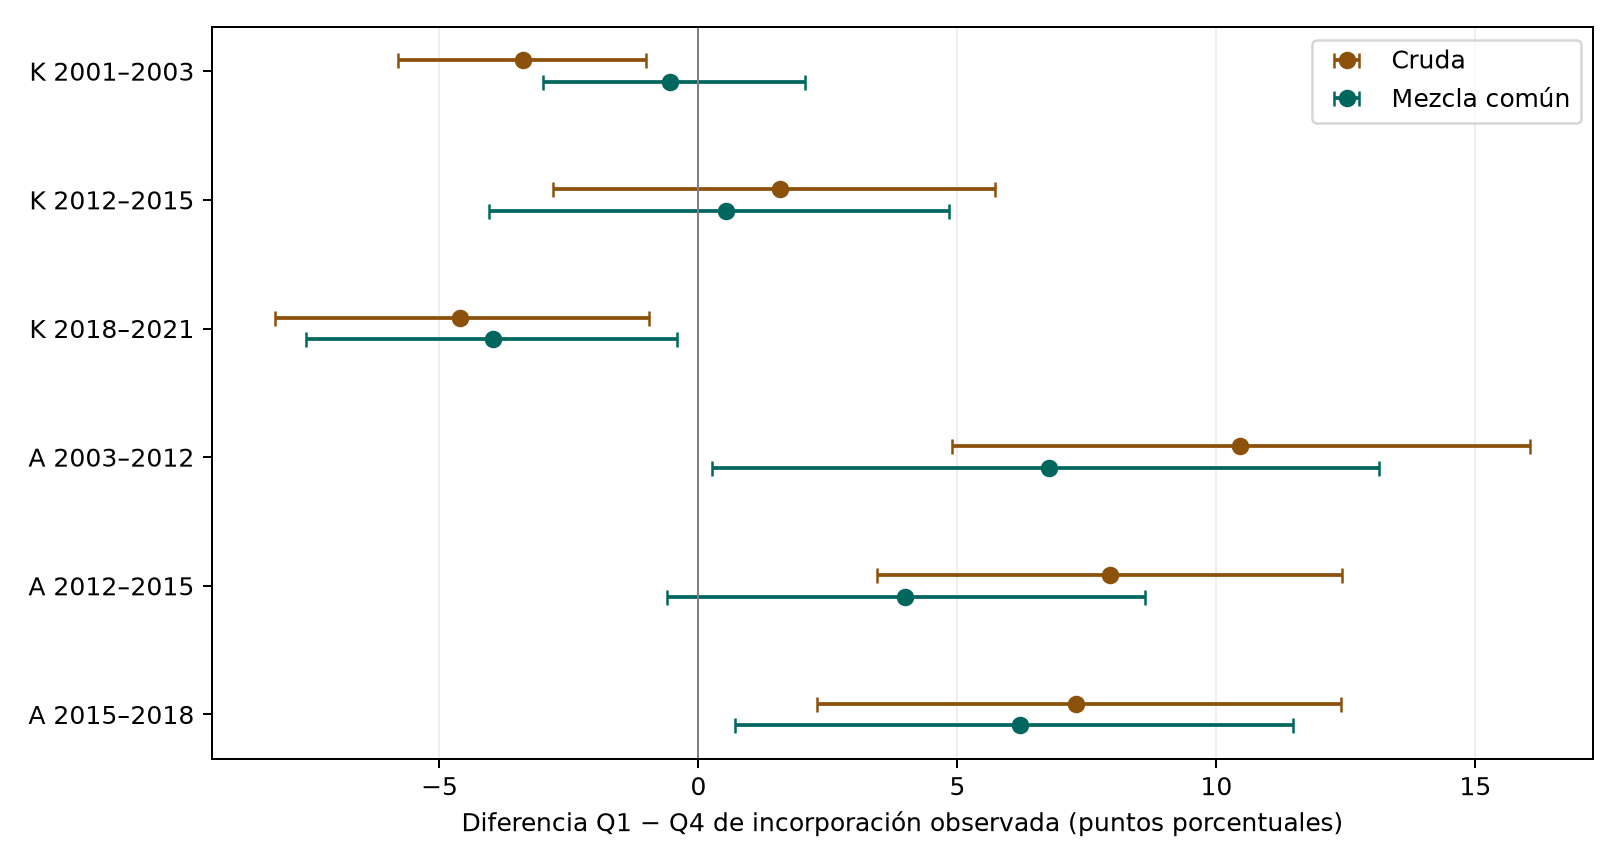
\includegraphics[width=.96\textwidth]{../resultados/figuras/central09_gradiente_patrimonio.png}\caption{Gradiente patrimonial de incorporación e IC95 condicionales por folio. Q1 menos Q4; mezcla común en soporte.}\label{fig:central-gradiente}\end{figure}
La asociación con menor patrimonio no es uniforme. Los gradientes crudos de A son positivos, pero A 2015--2018 incluye cero al cambiar a otra granularidad etaria con soporte adecuado, y A 2012--2015 incluye cero tras ajuste. A 2003--2012 mantiene señal positiva en variantes viables, con seguimiento selectivo. K no reproduce una preferencia uniforme por el menor patrimonio; K 2018--2021 conserva dirección puntual negativa con precisión sensible al soporte. Los cuadros de la sección de calidad del soporte muestran todas las especificaciones, sin elegir por significancia.

Dentro de K 2012--2015, P tiene patrimonio mediano mayor que C y menor que R, no el menor patrimonio de los tres perfiles. P es siete años más joven que C en mediana y tiene dos años más de escolaridad mediana; sus IC de diferencias por folio se conservan en el informe. En A 2015--2018, la diferencia patrimonial P menos C y la de escolaridad incluyen cero; P es seis años más joven. Son contraejemplos frente a equiparar primera vía con mayor necesidad. La localidad se conserva como corte 100 mil, sin llamarlo ruralidad.

\subsection{Importes posteriores y heterogeneidad}
\begingroup
\small\setlength{\tabcolsep}{4pt}
\begin{longtable}{lrrrrr}
\caption{Montos posteriores por protección basal y continuidad}\label{tab:central-montos}\\
\toprule
Vía/ventana & Perfil & N válido & Q25 & Mediana & Q75 \\
\midrule\endfirsthead
\multicolumn{6}{l}{\small Continuación del cuadro \thetable}\\
\toprule
Vía/ventana & Perfil & N válido & Q25 & Mediana & Q75 \\
\midrule\endhead
\bottomrule\endfoot
K 2001--2003 & P & 278 & 3,657.4 & 4,062.5 & 5,626.7 \\
K 2001--2003 & C & 11 & 3,376.0 & 3,376.0 & 6,189.4 \\
K 2001--2003 & R & 1,175 & 3,657.4 & 4,191.9 & 7,196.6 \\
K 2012--2015 & P & 1,060 & 941.5 & 1,027.1 & 3,937.2 \\
K 2012--2015 & C & 373 & 941.5 & 941.5 & 996.3 \\
K 2012--2015 & R & 1,857 & 3,423.6 & 4,279.6 & 10,270.9 \\
K 2018--2021 & P & 360 & 3,859.6 & 4,895.0 & 9,314.1 \\
K 2018--2021 & C & 132 & 2,107.6 & 4,079.2 & 5,234.9 \\
K 2018--2021 & R & 1,954 & 3,859.6 & 5,438.9 & 13,140.5 \\
A 2003--2012 & P & 666 & 962.2 & 962.2 & 1,443.3 \\
A 2003--2012 & C & 98 & 962.2 & 962.2 & 1,034.4 \\
A 2003--2012 & R & 278 & 962.2 & 962.2 & 1,732.0 \\
A 2012--2015 & P & 1,196 & 855.9 & 941.5 & 1,027.1 \\
A 2012--2015 & C & 286 & 855.9 & 941.5 & 1,690.4 \\
A 2012--2015 & R & 723 & 855.9 & 941.5 & 1,140.1 \\
A 2015--2018 & P & 581 & 840.6 & 886.5 & 1,299.2 \\
A 2015--2018 & C & 589 & 840.6 & 886.5 & 1,528.4 \\
A 2015--2018 & R & 1,245 & 840.6 & 886.5 & 1,528.4 \\
\end{longtable}
{\footnotesize Fuente: etapa 09, bases analíticas existentes y eventos originales, muestra no ponderada. P: ambas negativas basales; C: otra vía basal afirmativa; R: continuidad de la vía. No alta administrativa ni inferencia nacional. Pesos mensuales de septiembre de 2026, importe nominal multiplicado por factor del año calendario previo a entrevista real. Suma íntegra solo de eventos captados, no totalidad real. A incluye dinero/especie; no programa homogéneo. Diferencias de captura de la tabla 3.1 se mantienen.\par}
\endgroup

\begingroup\small\setlength{\tabcolsep}{3pt}
\begin{longtable}{lrrrrr}
\caption{Monto posterior por mitad patrimonial y protección basal}\label{tab:central-patrimonio_monto}\\
\toprule
Vía/ventana & Mitad & N P/C & Mediana P & Mediana C & P-C [IC95] \\
\midrule\endfirsthead
\multicolumn{6}{l}{Continuación del cuadro \thetable}\\
\toprule
Vía/ventana & Mitad & N P/C & Mediana P & Mediana C & P-C [IC95] \\
\midrule\endhead
\bottomrule\endfoot
K 2001--2003 & Inferior & Sin soporte & Reservado & Reservado & No estimable \\
K 2001--2003 & Superior & Sin soporte & Reservado & Reservado & No estimable \\
K 2012--2015 & Inferior & 553/230 & 992.9 & 941.5 & 51.4 [8.6; 68.5] \\
K 2012--2015 & Superior & 507/143 & 1,985.7 & 941.5 & 1,044.2 [492.1; 2,482.1] \\
K 2018--2021 & Inferior & 176/71 & 4,740.3 & 4,079.2 & 661.1 [37.7; 1,149.4] \\
K 2018--2021 & Superior & 184/61 & 5,438.9 & 4,079.2 & 1,359.7 [564.7; 2,175.6] \\
A 2003--2012 & Inferior & 372/42 & 962.2 & 962.2 & 0.0 [0.0; 0.0] \\
A 2003--2012 & Superior & 294/56 & 962.2 & 962.2 & 0.0 [0.0; 0.0] \\
A 2012--2015 & Inferior & 661/133 & 941.5 & 941.5 & 0.0 [0.0; 0.0] \\
A 2012--2015 & Superior & 535/153 & 941.5 & 941.5 & 0.0 [-51.4; 0.0] \\
A 2015--2018 & Inferior & 316/321 & 886.5 & 886.5 & 0.0 [-39.7; 7.6] \\
A 2015--2018 & Superior & 265/268 & 878.8 & 886.5 & -7.6 [-38.2; 34.4] \\
\end{longtable}
{\footnotesize Fuente: auditoría10, insumos01--09 intactos. Muestra sin ponderación; IC condicionales, sin inferencia nacional o causal. P: primera vía observada; C: otra vía basal afirmativa. Reformulación común Q1+Q2/Q3+Q4, manteniendo población, titularidad, ventanas y precios. 4999 réplicas por folio. K2001--2003 sigue sin soporte; retirar conjuntamente ambas mitades y derivados impide recuperar un importe mediante otra rama. No se escogió la agrupación por significancia.\par}
\endgroup

\begingroup
\small\setlength{\tabcolsep}{4pt}
\begin{longtable}{lrrrr}
\caption{Diferencia de medianas posteriores: P menos C}\label{tab:central-diferencias}\\
\toprule
Vía/ventana & N P/C & Cruda [IC95] & Mezcla común [IC95] & Retención \% \\
\midrule\endfirsthead
\multicolumn{5}{l}{\small Continuación del cuadro \thetable}\\
\toprule
Vía/ventana & N P/C & Cruda [IC95] & Mezcla común [IC95] & Retención \% \\
\midrule\endhead
\bottomrule\endfoot
K 2001--2003 & 278/11 & No estimado & No estimado & 0/0 \\
K 2012--2015 & 1\,060/373 & 85{,}6 [51{,}4; 409{,}8] & No estimado & 57/90 \\
K 2018--2021 & 360/132 & 815{,}8 [543{,}9; 1\,324{,}3] & No estimado & 20/50 \\
A 2003--2012 & 666/98 & 0{,}0 [0{,}0; 0{,}0] & No estimado & 0/0 \\
A 2012--2015 & 1\,196/286 & 0{,}0 [0{,}0; 0{,}0] & No estimado & 51/79 \\
A 2015--2018 & 581/589 & 0{,}0 [-30{,}6; 7{,}6] & -7{,}6 [-38{,}2; 7{,}6] & 73/89 \\
\end{longtable}
{\footnotesize Fuente: elaboración propia con las bases analíticas y eventos originales de ENASEM; muestra no ponderada. P: ambas negativas basales; C: otra vía basal afirmativa; R: continuidad de la vía. No alta administrativa ni inferencia nacional. Pesos reales. Crudo: bootstrap folio 4999. Mezcla común: sexo por edad de tres grupos por escolaridad 0--5/6+, 1999 réplicas y CDF inversa. Mínimo 20 por grupo/celda, 4 celdas y 70\% de cada grupo completo antes de excluir covariables ND. No estimado si falta soporte; no se extrapola. Crudo y ajustado pueden usar poblaciones y convenciones distintas; crudo del mismo soporte en agregados. Los empates y la concentración de importes pueden producir extremos repetidos o IC de amplitud cero en el bootstrap de medianas; no implican certeza absoluta, igualdad distributiva ni ausencia de incertidumbre.\par}
\endgroup

\begingroup
\small\setlength{\tabcolsep}{4pt}
\begin{longtable}{llrr}
\caption{Heterogeneidad institucional del contraste P menos C}\label{tab:central-instituciones}\\
\toprule
Vía/ventana & Evidencia destino & N P/C & Diferencia real [IC95] \\
\midrule\endfirsthead
\multicolumn{4}{l}{\small Continuación del cuadro \thetable}\\
\toprule
Vía/ventana & Evidencia destino & N P/C & Diferencia real [IC95] \\
\midrule\endhead
\bottomrule\endfoot
K 2012--2015 & IMSS/ISSSTE & 406/27 & 513{,}5 [0{,}0; 984{,}3] \\
K 2012--2015 & Programa agrupado & 599/326 & 0{,}0 [0{,}0; 0{,}0] \\
K 2012--2015 & Un evento IMSS & 305/20 & 428{,}0 [0{,}0; 684{,}7] \\
K 2018--2021 & IMSS/ISSSTE & 309/79 & 679{,}9 [-40{,}0; 1\,087{,}8] \\
K 2018--2021 & Un evento IMSS & 259/68 & 271{,}9 [-193{,}1; 679{,}9] \\
A 2015--2018 & A: INAPAM & 163/155 & -30{,}6 [-45{,}9; 34{,}4] \\
A 2015--2018 & A: Otra institución & 217/257 & 0{,}0 [-7{,}6; 7{,}6] \\
A 2015--2018 & A: PROSPERA & 149/119 & -15{,}3 [-45{,}9; 30{,}6] \\
\end{longtable}
{\footnotesize Fuente: elaboración propia con las bases analíticas y eventos originales de ENASEM; muestra no ponderada. P: ambas negativas basales; C: otra vía basal afirmativa; R: continuidad de la vía. No alta administrativa ni inferencia nacional. IC folio 1999. Evidencia K puede solaparse: no sumar filas ni asignar el importe a cada institución. Un evento exige un solo evento captado; IMSS/ISSSTE no identifica régimen. A solo 2018: nombres reportados, no programa longitudinal homologado ni A5 retrospectivo. Celdas inferiores a 20 no generan IC. Los empates y la concentración de importes pueden producir IC de amplitud cero en el bootstrap de medianas; no implican certeza absoluta, igualdad distributiva ni ausencia de incertidumbre.\par}
\endgroup


\begin{figure}[htbp]\centering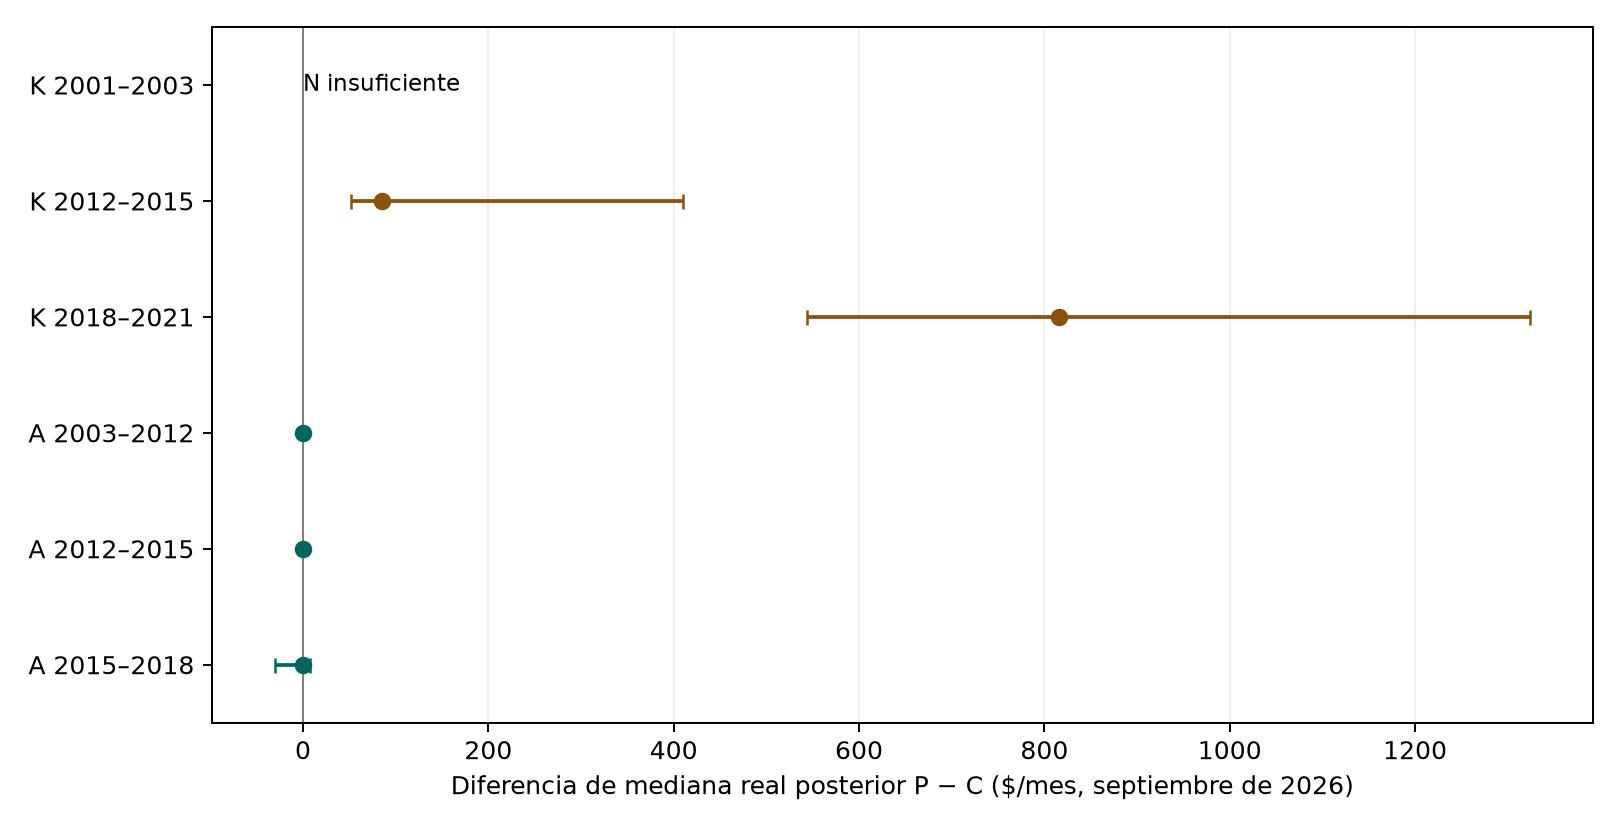
\includegraphics[width=.96\textwidth]{../resultados/figuras/central09_diferencias_montos.png}\caption{Diferencias de medianas posteriores P menos C, pesos mensuales de septiembre de 2026; IC95 por folio.}\label{fig:central-dinero}\end{figure}
En K 2012--2015 y 2018--2021, P tiene una mediana posterior mayor que C; los IC crudos por folio excluyen cero. En 2001--2003 el perfil C solo contiene 12 receptores y 11 montos válidos: se describe, sin IC comparativo. En la definición original, las tres ventanas A comparten la misma mediana P/C en cada destino. Sus IC describen empates, sin demostrar equivalencia económica o distribuciones iguales.

El cuadro~\ref{tab:central-patrimonio_monto}, organizado en mitades patrimoniales, cruza las tres dimensiones de la pregunta: patrimonio inicial, protección previa y monto posterior. No basta con comparar el patrimonio de grupos por un lado y los montos por otro. Los estratos de baja frecuencia se describen sin IC y no se eliminan porque limiten la hipótesis.

La composición importa: en K 2012--2015 el contraste P menos C es mucho mayor entre hombres que entre mujeres y entre 60--64 que entre 70+. Los contrastes por sexo, escolaridad y localidad se sintetizan a continuación; diferencias de intervalos entre estratos no se interpretan como prueba formal de interacción. En A 2015--2018, la estandarización monetaria viable sigue produciendo un contraste cercano a cero. En las restantes ventanas falta soporte para una mediana P/C estandarizada que retenga 70\% de ambos perfiles. No se extrapola el ajuste de nuevos frente a continuos a este contraste diferente.

En la definición original, la evidencia IMSS/ISSSTE atenúa la precisión del contraste P/C en las ventanas K recientes: sus IC incluyen cero. En el código de programas agrupados K 2012--2015 coinciden las medianas. Estas filas pueden solaparse y sus importes no se reparten por institución. Para A solo se desglosan nombres captados al destino 2018 y personas con un evento: ello describe heterogeneidad del destino, sin reconstruir programas previos, A5 o identidad administrativa.

\subsection{Selección, desconocidos y coexistencia}
\begingroup
\small\setlength{\tabcolsep}{4pt}
\begin{longtable}{lrrrrr}
\caption{Seguimiento de cohortes negativas y límites de observación}\label{tab:central-seleccion}\\
\toprule
Vía/ventana & Perfil & N basal & Fallecido & Ausente & Cota \% sin D \\
\midrule\endfirsthead
\multicolumn{6}{l}{\small Continuación del cuadro \thetable}\\
\toprule
Vía/ventana & Perfil & N basal & Fallecido & Ausente & Cota \% sin D \\
\midrule\endhead
\bottomrule\endfoot
K 2001--2003 & P & 4,533 & 239 & 223 & 6.7--19.6 \\
K 2001--2003 & C & 576 & 22 & 22 & 2.2--18.8 \\
K 2012--2015 & P & 4,592 & 319 & 199 & 25.5--35.6 \\
K 2012--2015 & C & 1,323 & 145 & 26 & 31.9--41.7 \\
K 2018--2021 & P & 3,368 & 304 & 184 & 12.5--24.4 \\
K 2018--2021 & C & 2,422 & 337 & 55 & 6.6--19.2 \\
A 2003--2012 & P & 4,368 & 1,165 & 400 & 21.2--46.6 \\
A 2003--2012 & C & 1,631 & 504 & 201 & 8.7--36.8 \\
A 2012--2015 & P & 4,592 & 319 & 199 & 28.3--38.2 \\
A 2012--2015 & C & 2,562 & 214 & 150 & 12.6--23.6 \\
A 2015--2018 & P & 3,253 & 194 & 374 & 19.7--38.1 \\
A 2015--2018 & C & 3,622 & 273 & 382 & 18.1--36.4 \\
\end{longtable}
{\footnotesize Fuente: etapa 09, bases analíticas existentes y eventos originales, muestra no ponderada. P: ambas negativas basales; C: otra vía basal afirmativa; R: continuidad de la vía. No alta administrativa ni inferencia nacional. Cota sin D: entre quienes no tienen fallecimiento registrado, incorporar a todos los destinos no clasificables o a ninguno. No acredita que ausentes estén vivos ni incidencia previa a morir. Fallecimientos quedan separados, sin imputar recepción post mortem. Sustitutos, ND y conflictos separados en informe y agregados.\par}
\endgroup


Las cotas de seguimiento son amplias y no son IC de muestreo: responden a falta de observación, no a la precisión de una mediana entre observados. El informe conserva las particiones exhaustivas de toda cohorte, los perfiles de cada destino, los montos faltantes y las sensibilidades por sustituto, edad final y fecha de precios. Sus resultados no recuperan las trayectorias no observadas. Entre receptores observados, las cotas por importes faltantes mantienen positiva la diferencia mediana P menos C en K 2012--2015 y 2018--2021; no son IC y no incluyen selección de ausentes o fallecidos. Los intervalos exactos permanecen en el informe.

En K 2012--2015, de 376 incorporados con A basal, 130 declaran A al destino, 244 la niegan y 2 son ND. La complementariedad basal no implica acumulación al final: el estado C incluye también pérdida o cambio de declaración de la otra vía, sin acreditar sustitución administrativa.

La otra vía basal no demuestra coexistencia simultánea. El informe tabula afirmativa, negativa y ND de la otra vía al destino para P y C; solo 2012--2015 admite interpretación longitudinal conjunta. En las demás ventanas, esa respuesta de destino es descripción bajo su propio cuestionario. La persistencia sin ambas vías se cuantifica conjuntamente solo donde ambas son comparables. No se interpreta una ruptura como aparición o desaparición económica real.

\subsection{Sensibilidad de la medición y alcance de primera vía}
\label{sec:resultados-sensibilidad-medicion}

Los cuadros~\ref{tab:sensibilidad-medicion-k}--\ref{tab:sensibilidad-ventanas}
conservan la definición original y la alternativa estricta de la
sección~\ref{sec:sensibilidad-medicion}. En K 2012--2015, nuevos receptores
pasan de 1\,469 a 539; P de 1\,090 a 489 y C de 376 a 49. Los demás no se
reclasifican como personas sin recursos, sino como no comparables bajo el
criterio alternativo. En A no cambia la incorporación total, pero sí la
identificación de K basal: C pasa de 296 a 166 en 2012--2015 y de 606 a 153
en 2015--2018. No se demuestra que toda esta diferencia provenga de una
reclasificación real de un mismo programa.

Manteniendo el denominador original de reobservados K, la incorporación
conocida sin 08 es 489/3\,843 entre P, 12{,}72\% (IC95\% por folio:
11{,}69--13{,}84\%), y 49/1\,063 entre C, 4{,}61\% (3{,}32--6{,}00\%).
El orden es opuesto al de la recepción K original, 28{,}36 frente a
35{,}37\%. Se trata de un resultado institucional distinto sobre los mismos
denominadores, no de un efecto de A sobre K ni de una tasa administrativa.
El denominador K no coincide necesariamente con el de unión, porque una
A afirmativa puede resolver esta última aunque K sea desconocida.

En el subgrupo con evidencia IMSS/ISSSTE de destino, apartar solo 08
identificado en las visitas necesarias deja 391/25 montos P/C frente a
406/27 originales. El punto P--C es 513{,}55 en ambos casos; los IC95\%
con 4\,999 réplicas por folio y semilla 20261024 son [171{,}18; 855{,}91]
y [0; 1\,027{,}09], respectivamente. Los C de 25/27 válidos son exploratorios;
no se escoge el intervalo que excluye cero como explicación institucional.
El contraste de un evento IMSS, con 305/20, conserva 427{,}96 [0; 684{,}73].
La rama de un evento ISSSTE no tiene soporte para un contraste. La evidencia
institucional puede ser múltiple y no asigna el importe a una institución.

La diferencia monetaria nuevos menos continuos K pasa de -3\,286{,}70 a
-513{,}55 pesos reales en la alternativa estricta; P menos C pasa de
85{,}59 a 1\,027{,}09. Sus IC y N válidos figuran en el
cuadro~\ref{tab:sensibilidad-medicion-k}. Las magnitudes dependen de la
mezcla institucional. Tener otra vía al inicio no explica causalmente
la diferencia ni acredita un incremento de ingreso total.

La historia previa aporta otro límite: 217 de las 1\,090 personas P de
K 2012--2015 y 148 de las 384 de K 2018--2021 tenían alguna declaración
K/A positiva en una entrevista directa anterior sin conflicto vital. En
A 2012--2015 son 222/1\,210 y en A 2015--2018, 149/603. Esas declaraciones
se leen bajo el cuestionario de cada ronda, sin validar puentes excluidos.
P significa primera vía desde ambas negativas en esa pareja de rondas,
no primera recepción conocida en toda la historia ni de toda la vida.

\paragraph{Patrimonio y magnitud.}
La interacción entre contrastes de mitades patrimoniales K 2012--2015
es 992{,}86 pesos reales, IC95\% [666{,}97; 2\,430{,}79] en la definición
original. Al apartar solo 08 identificado es -684{,}73
[-1\,883{,}01; 3\,595{,}26], con grupos C de 20 y 27 válidos, exploratorios.
El cuadro~\ref{tab:sensibilidad-interaccion} muestra que la heterogeneidad
por patrimonio no es robusta a esta decisión de medición; el signo alternativo
no demuestra una reversión poblacional. Los N de 20 y 27 cuentan personas C
con monto posterior íntegro válido en las mitades basal inferior y superior,
respectivamente; no son frecuencias en la mediana ni números de folios.
El cambio de signo puede reflejar tanto la reclasificación institucional
como la inestabilidad de muestras reducidas; esta sensibilidad no separa
sus contribuciones. No sustenta una conclusión general sobre patrimonio.
En K 2018--2021 la interacción también incluye
cero, aunque los dos contrastes por mitad sean positivos. No basta comparar
sus significancias por separado.

El contraste original K 2012--2015 P--C de 85{,}59 equivale aproximadamente
al 9{,}1\% de la mediana C de 941{,}50; por mitad patrimonial son 5{,}5\% y
110{,}9\%. La precisión no vuelve equivalentes esas magnitudes ni establece
su suficiencia económica. El patrimonio compartido tampoco mide necesidad.

\paragraph{Composición y soporte.}
En K 2012--2015 los N válidos P/C son 478/160 en hombres y 582/213 en
mujeres; los contrastes son 1\,112{,}69 [770{,}32; 2\,482{,}14] y
51{,}35 [8{,}56; 51{,}35]. Con escolaridad basal de cero años,
233/152: 0 [0; 42{,}80]; de 1--5 años, 377/162: 51{,}35 [0; 51{,}35];
con seis años, 249/40: 834{,}51 [34{,}24; 2\,439{,}35]. En localidades
menores de 100 mil habitantes, 486/304: 42{,}80 [17{,}12; 51{,}35]; en las
mayores, 574/69: 2\,054{,}19 [1\,027{,}09; 2\,430{,}79]. Son IC95\%
por folio con 1\,999 réplicas, semilla 20261024, sin ajuste ni prueba formal
de interacción. Los restantes estratos educativos carecen de soporte; no se
utilizan para conclusiones monetarias.

La estandarización monetaria P/C K 2012--2015 no es viable en ninguna de las
cuatro configuraciones de edad y mínimos por celda examinadas. La alternativa
que más se aproxima conserva solo 69{,}72\% de P, por debajo del 70\%
exigido; no se redondea para aceptar el ajuste. El gradiente patrimonial
Q1 menos Q4 de incorporación K, restringido a solo 08 identificado, pasa de
-3{,}95 puntos porcentuales crudos [-7{,}43; -0{,}44] a -1{,}41
[-5{,}08; 2{,}53] al estandarizar sexo, edad y escolaridad, con soporte
749/774 y 1\,999 réplicas, semilla 20261024. La asociación cruda no se
mantiene inequívocamente tras considerar composición.

\paragraph{Atrición e identificación de la unión.}
La fracción detectada original es 2\,188/4\,592, 47{,}65\%; no es una
estimación corregida de incorporación en la cohorte. Excluyendo únicamente
319 defunciones registradas, quedan 4\,273 personas sin esa condición y 427
destinos no clasificables; los límites son 51{,}21--61{,}20\%. No certifican
que los ausentes estén vivos, ni constituyen IC. En la alternativa estricta,
1\,643/3\,301 = 49{,}77\% entre clasificables alternativos; sobre los
3\,846 observados originales se identifica 42{,}72\% y los 545 ND adicionales
permiten límites de medición 42{,}72--56{,}89\%. No hay una única tasa
``corregida'' que reemplace el 56{,}9\% original.

De los 376 incorporados K con A basal, los 130 que conservan A y los 244 que
la niegan incluyen, respectivamente, 109 y 216 con 08 en K. Esto respalda
examinar medición, pero no identifica el beneficio administrativo. Los pares
monetarios válidos A origen/K destino son 127/237, en 117/213 folios. Las
medianas de diferencias reales individuales son -20{,}69 en ambos conjuntos,
IC95\% [-20{,}69; 85{,}65] y [-20{,}69; 22{,}10], con 4\,999 réplicas,
semilla 20261023. A puede incluir especie; esos cambios no son ganancias o
pérdidas del ingreso total ni prueba de continuidad de un programa.


% END central09_resultados
\FloatBarrier
\section*{Contexto descriptivo y contrastes complementarios}
Los resultados siguientes sitúan el contraste central en las seis rondas;
no sustituyen la respuesta sobre incorporación desde negativas basales.

\section{Distribución y superposición de vías propias}
\label{sec:resultados-cobertura}

El cuadro~\ref{tab:tesis-cobertura} distingue recepción propia K, apoyo
propio A y unión de ambas vías entre personas vivas de 60 años o más con
entrevista directa. Cada tasa conserva su denominador conocido y cada
fila corresponde a un corte. Las diferencias de cobertura entre filas que
atraviesan rupturas no se interpretan como una trayectoria homologada.

La selección de ventanas se fundamenta en la
sección~\ref{sec:comparabilidad-ventanas} y el
cuadro~\ref{tab:comparabilidad-ventanas}. Se mantienen los seis cortes
descriptivos incluso donde no se admite transición homologada.
En particular, el cambio A 2018--2021 no estima incorporaciones reales
de una definición invariable; A 2001--2003 mantiene homologación pendiente.

% Exportado desde agregados; no editar cifras manualmente.
\begin{table}[!htbp]
\centering
\caption{Recepción propia y estados de información por ronda, directas 60+, 2001--2021}\label{tab:tesis-cobertura}
\footnotesize\setlength{\tabcolsep}{3pt}\renewcommand{\arraystretch}{1.25}
\begin{tabularx}{\linewidth}{p{.075\linewidth}p{.085\linewidth}YYYp{.135\linewidth}p{.13\linewidth}}
\toprule
\textbf{Ronda} & \textbf{N elegible} & \textbf{K: \% (N)} & \textbf{A: \% (N)} & \textbf{Unión: \% (N)} & \textbf{ND K/A/unión} & \textbf{Ambas negativas} \\
\midrule
2001 & 6\,812 & \ensuremath{24,74}\ \allowbreak\ensuremath{(6\,790)} & \ensuremath{9,81}\ \allowbreak\ensuremath{(6\,789)} & \ensuremath{33,23}\ \allowbreak\ensuremath{(6\,789)} & 22/\allowbreak{}23/\allowbreak{}23 & 4\,533 \\
2003 & 6\,970 & \ensuremath{25,53}\ \allowbreak\ensuremath{(6\,894)} & \ensuremath{12,98}\ \allowbreak\ensuremath{(6\,894)} & \ensuremath{36,64}\ \allowbreak\ensuremath{(6\,894)} & 76/\allowbreak{}76/\allowbreak{}76 & 4\,368 \\
2012 & 8\,888 & \ensuremath{32,26}\ \allowbreak\ensuremath{(8\,738)} & \ensuremath{17,99}\ \allowbreak\ensuremath{(8\,750)} & \ensuremath{47,42}\ \allowbreak\ensuremath{(8\,734)} & 150/\allowbreak{}138/\allowbreak{}154 & 4\,592 \\
2015 & 9\,640 & \ensuremath{43,76}\ \allowbreak\ensuremath{(9\,504)} & \ensuremath{27,65}\ \allowbreak\ensuremath{(9\,513)} & \ensuremath{65,79}\ \allowbreak\ensuremath{(9\,508)} & 136/\allowbreak{}127/\allowbreak{}132 & 3\,253 \\
2018 & 9\,107 & \ensuremath{35,89}\ \allowbreak\ensuremath{(9\,047)} & \ensuremath{30,56}\ \allowbreak\ensuremath{(9\,045)} & \ensuremath{62,74}\ \allowbreak\ensuremath{(9\,039)} & 60/\allowbreak{}62/\allowbreak{}68 & 3\,368 \\
2021 & 9\,424 & \ensuremath{34,82}\ \allowbreak\ensuremath{(9\,366)} & \ensuremath{52,59}\ \allowbreak\ensuremath{(9\,363)} & \ensuremath{67,97}\ \allowbreak\ensuremath{(9\,366)} & 58/\allowbreak{}61/\allowbreak{}58 & 3\,000 \\
\bottomrule
\end{tabularx}
\notacuadro{Cada tasa usa el N conocido entre paréntesis; ND se cuenta sobre el N elegible de la fila y no significa negativa. Unión: alguna afirmativa; no: ambas negativas. K y A se superponen. Las filas son cortes separados, no una serie homogénea a través de rupturas K 2003--2012/K 2015--2018 o A 2001--2003/A 2018--2021.}
\fuentecuadro{Elaboración propia, ENASEM; agregados de notebooks 06--08 y validación focalizada del informe general, secciones 10.2--10.7. Sin ponderación nacional.}
\end{table}

\FloatBarrier

La superposición de K y A implica que sus porcentajes no son aditivos.
Una afirmativa basta para identificar alguna vía propia; clasificar la
combinación exclusiva requiere información adicional. Este criterio explica
que el N de unión conocida pueda exceder el de ambas recepciones conocidas.
En 2021, dentro del grupo de 70 años o más con entrevista directa,
4\,733/5\,099 con unión conocida declaran recepción, 92{,}82\%; el total
es 5\,125, con 26 ND. No es una estimación nacional ni un indicador de
suficiencia económica integral. La información del cónyuge se analiza como contexto y no aumenta la cobertura
propia por asignación automática.

En 2021, \dato{2021.N_KA_si} de \dato{2021.N_KA_conocido} personas con unión
conocida reportan al menos una vía propia (\dato{2021.KA}\%).
Hay \dato{2021.N_KA_no} negativas explícitas de ambas vías y
\dato{2021.N_KA_ND_elegible} estados de unión desconocida entre
\dato{2021.N_elegible} directas elegibles. Son estados diferentes:
las negativas no demuestran ausencia de todos los recursos económicos
y los desconocidos no se añaden a las negativas.

La tipología documentada identifica 538 directas con pareja confirmada y
solo K del cónyuge, con negativas propias K/A; otras 884 tienen negativas
propias y ausencia explícita de pareja residente. Ambos grupos forman parte
de las negativas propias, pero su contexto difiere. En el primero no se
conoce el reparto efectivo del dinero del cónyuge; en el segundo no se
infiere que falte todo apoyo familiar. Esta distinción responde a quiénes
no tienen una vía propia identificada, sin convertirla en clasificación
de pobreza o dependencia económica completa.

\section{Brechas de cobertura por características socioeconómicas}
\label{sec:resultados-perfiles}

Las diferencias de acceso no tienen la misma dirección para todas las vías.
En 2021, la unión es \dato{Perfil.SinEscuela.Union}\% entre quienes no
registran escolaridad (\dato{Perfil.SinEscuela.UnionSi}/\dato{Perfil.SinEscuela.UnionN}),
frente a \dato{Perfil.AltaEscuela.Union}\% con al menos diez años
(\dato{Perfil.AltaEscuela.UnionSi}/\dato{Perfil.AltaEscuela.UnionN}).
No se concluye que el primer grupo tenga mejores recursos:
la comparación monetaria de la sección~\ref{sec:resultados-brechas-monto}
muestra un contraste diferente.

Por edad, la unión pasa de \dato{Perfil.EdadTemprana.Union}\% en 60--64
(\dato{Perfil.EdadTemprana.UnionSi}/\dato{Perfil.EdadTemprana.UnionN})
a \dato{Perfil.EdadMayor.Union}\% en 70+
(\dato{Perfil.EdadMayor.UnionSi}/\dato{Perfil.EdadMayor.UnionN}).
Es una comparación entre perfiles contemporáneos, no un aumento de esa
magnitud al envejecer la misma persona. Las reglas de edad, la generación,
la recepción previa y la supervivencia no se separan causalmente.

En localidades menores de 100 mil habitantes, la unión alcanza
\dato{Perfil.LocalidadMenor.Union}\%
(\dato{Perfil.LocalidadMenor.UnionSi}/\dato{Perfil.LocalidadMenor.UnionN}),
frente a \dato{Perfil.LocalidadMayor.Union}\%
(\dato{Perfil.LocalidadMayor.UnionSi}/\dato{Perfil.LocalidadMayor.UnionN})
en las mayores. El corte no identifica ruralidad estricta y la proximidad
de tasas de unión no prueba igualdad de recursos o necesidades.

La brecha hombre--mujer requiere distinguir el nivel de cada corte del
cambio entre ellos. En 2012--2015, la diferencia de cobertura de unión
se reduce, mientras la diferencia K aislada no presenta un cambio preciso.
Los intervalos y denominadores aparecen conjuntamente con la brecha monetaria
en el cuadro~\ref{tab:tesis-sexo}. La ocupación se mantiene como perfil
descriptivo en los agregados: no se interpreta retirado/incapacitado/no
trabaja como una categoría homogénea de pensionados ni se añade un modelo
laboral explicativo.

\section{Evolución de montos nominales y reales}
\label{sec:resultados-montos}

El cuadro~\ref{tab:tesis-montos} conserva el nivel nominal y el poder
adquisitivo común de los importes captados. El número de receptoras y
receptores es mayor que el N con monto válido. Los cuantiles de los
cortes responden a sus distribuciones disponibles y no a un panel de
beneficiarios fijos.

% Exportado desde agregados; no editar cifras manualmente.
\begin{table}[!htbp]
\centering
\caption{Montos mensuales captados y referencia económica, directas 60+, 2001--2021}\label{tab:tesis-montos}
\footnotesize\setlength{\tabcolsep}{3pt}\renewcommand{\arraystretch}{1.25}
\begin{tabularx}{\linewidth}{p{.075\linewidth}p{.04\linewidth}YYYYY}
\toprule
\textbf{Ronda} & \textbf{Vía} & \textbf{N recibe} & \textbf{N nom./real} & \textbf{Mediana nominal (\$)} & \textbf{Mediana real (\$)} & \textbf{Prestación/ LPI: mediana \% (N)} \\
\midrule
2001 & K & 1\,680 & 1\,608/\allowbreak{}1\,608 & 1\,227,00 & 3\,856,54 & 80,38 (1\,170) \\
2003 & K & 1\,760 & 1\,714/\allowbreak{}1\,714 & 1\,490,00 & 4\,191,92 & 86,62 (1\,247) \\
2012 & K & 2\,819 & 2\,633/\allowbreak{}2\,633 & 2\,200,00 & 4\,233,66 & 92,84 (2\,632) \\
2015 & K & 4\,159 & 3\,965/\allowbreak{}3\,965 & 2\,200,00 & 3\,766,01 & 78,22 (3\,963) \\
2018 & K & 3\,247 & 2\,994/\allowbreak{}2\,994 & 2\,800,00 & 4\,279,56 & 95,58 (2\,994) \\
2021 & K & 3\,261 & 3\,062/\allowbreak{}3\,062 & 4\,000,00 & 5\,438,89 & 119,49 (3\,062) \\
2001 & A & 666 & 625/\allowbreak{}625 & 200,00 & 628,61 & 20,39 (81) \\
2003 & A & 895 & 821/\allowbreak{}821 & 250,00 & 703,34 & 28,87 (142) \\
2012 & A & 1\,574 & 1\,535/\allowbreak{}1\,534 & 500,00 & 962,20 & 24,09 (1\,533) \\
2015 & A & 2\,630 & 2\,582/\allowbreak{}2\,582 & 550,00 & 941,50 & 20,76 (2\,582) \\
2018 & A & 2\,764 & 2\,699/\allowbreak{}2\,699 & 580,00 & 886,48 & 20,47 (2\,699) \\
2021 & A & 4\,924 & 4\,883/\allowbreak{}4\,883 & 1\,550,00 & 2\,107,57 & 43,66 (4\,883) \\
2021 & A5 & 4\,784 & 4\,758/\allowbreak{}4\,758 & 1\,550,00 & 2\,107,57 & 43,66 (4\,758) \\
\bottomrule
\end{tabularx}
\notacuadro{K/A: suma personal observada parcial, no ingreso total. A5: evento explícito de vejez; no se añade de nuevo a A. Pesos reales de septiembre de 2026, precios del año calendario anterior a entrevista real. LPI por persona/mes del mismo periodo: la razón se calcula individualmente antes de resumir. En 2001/2003 solo localidades de al menos 100 mil habitantes tienen ámbito asignable; su N de LPI no es comparable con el total posterior. Una prestación bajo LPI no clasifica pobreza.}
\fuentecuadro{Elaboración propia, ENASEM; agregados de notebooks 06--08 y validación focalizada del informe general, secciones 10.2--10.7. Sin ponderación nacional.}
\end{table}

\FloatBarrier

En K 2012--2015, las medianas nominales son
\$\dato{K.2012.Nominal} y \$\dato{K.2015.Nominal}; las reales pasan de
\$\dato{K.2012.Real} a \$\dato{K.2015.Real}, con
\dato{K.2012.N}/\dato{K.2015.N} importes válidos.
El nivel nominal central sin aumento no mantiene su poder adquisitivo.
La igualdad nominal de 2\,200 pesos no implica igualdad distributiva:
Q25/Q75 son 1\,800/5\,000 en 2012 y 600/4\,000 en 2015. La diferencia
de medianas reales entre cortes es -467{,}65, IC95\% [-467{,}65; -275{,}21],
con 2\,633/3\,965 montos válidos, 4\,836 personas y 4\,225 folios.
Se usan 4\,999 réplicas conjuntas por folio, semilla 20261024;
no es una pérdida de las mismas personas.
Al mismo tiempo, el cuadro~\ref{tab:tesis-cobertura} muestra más recepción K.
Esta coexistencia es compatible con H1 en esa ventana; no identifica
qué parte del cambio se debe a cada componente de la mezcla de receptores.

En A 2015--2018, la mediana nominal pasa de
\$\dato{A.2015.Nominal} a \$\dato{A.2018.Nominal}, pero la real cambia de
\$\dato{A.2015.Real} a \$\dato{A.2018.Real}, con
\dato{A.2015.N}/\dato{A.2018.N} montos válidos.
La diferencia de medianas reales entre estos cortes A es -55{,}02,
IC95\% [-55{,}02; -55{,}02], con 2\,582/2\,699 válidos, 4\,041 personas y
3\,341 folios; 4\,999 réplicas conjuntas, semilla 20261024. La degeneración
del IC refleja acumulaciones de importes, no ausencia de incertidumbre de
medición o selección. La recepción A aumenta en una ventana con
comparabilidad condicionada.
El incremento de pesos declarados no constituye una mejora real de la
mediana. A incluye dinero y especie y cambia su captación por eventos;
no se atribuye todo el patrón a una prestación federal.

\begin{landscape}
\begin{figure}[p]
\centering
\caption{Cobertura y poder adquisitivo en las ventanas K 2012--2015 y A 2015--2018}
\label{fig:tesis-cobertura-monto}
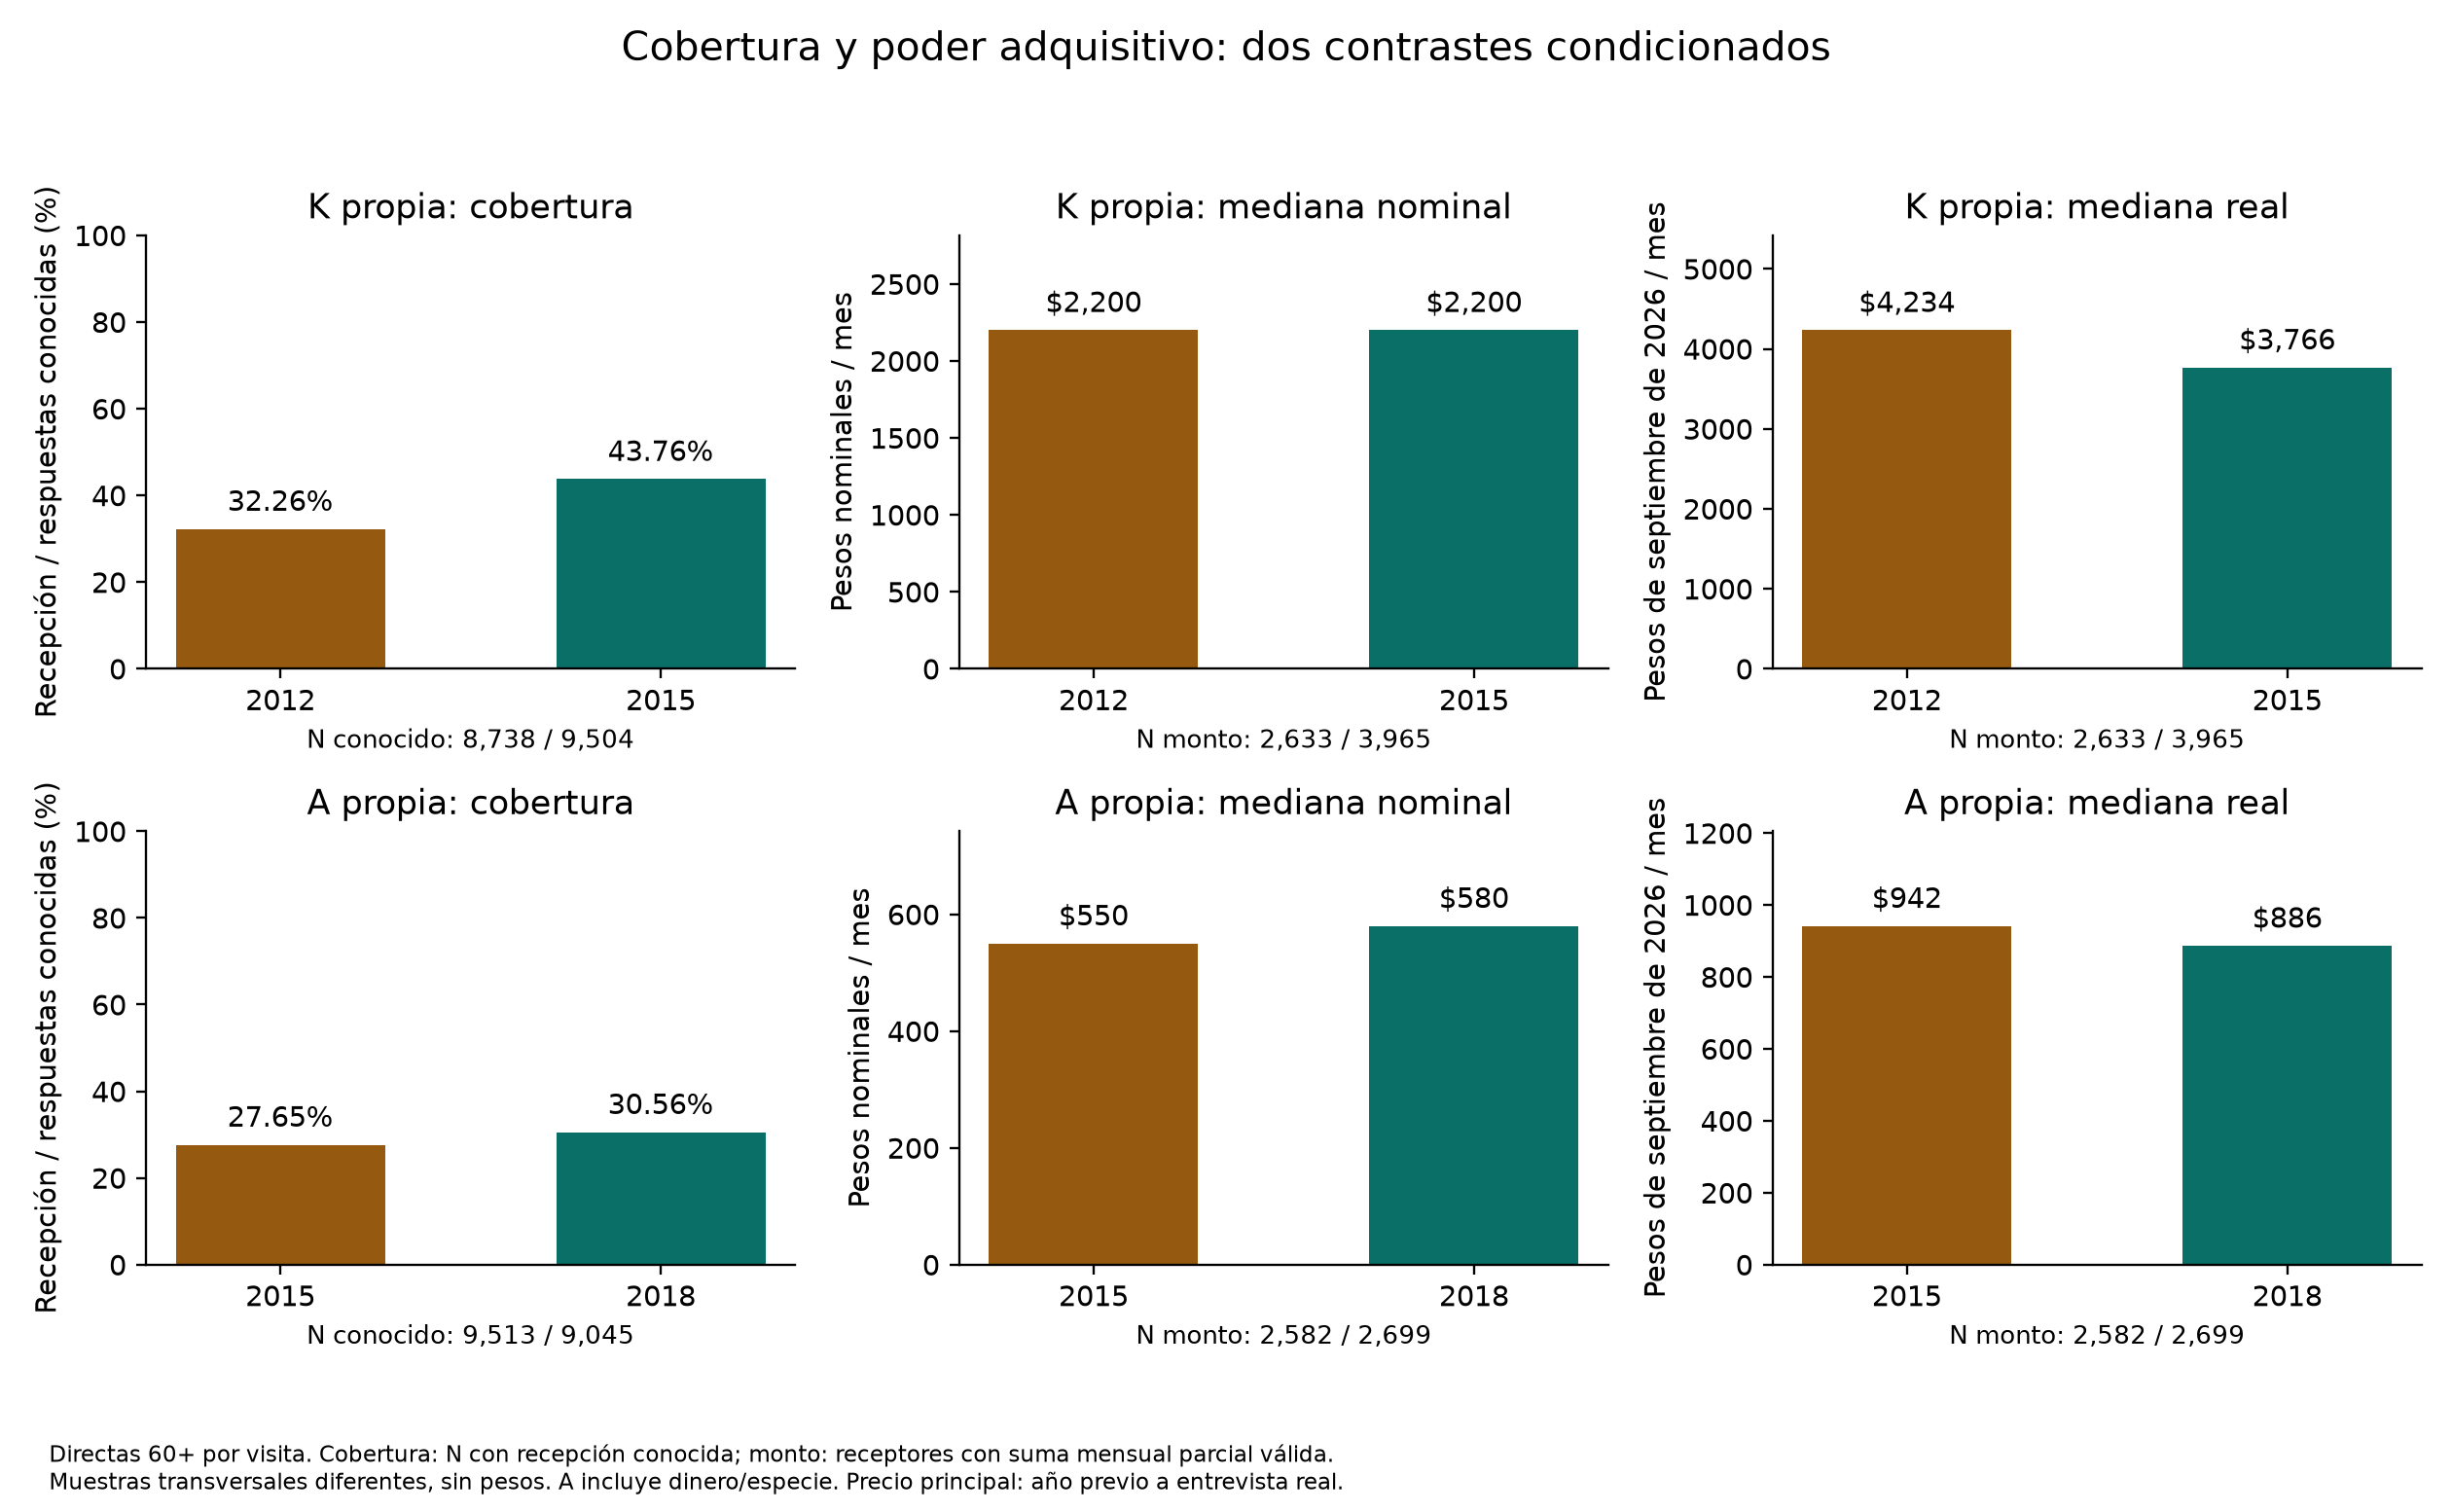
\includegraphics[width=\linewidth,height=.72\textheight,keepaspectratio]{../resultados/figuras/sintesis_proteccion__cobertura_poder_adquisitivo.png}
\notacuadro{Directas 60+ de cada visita; tasas entre respuestas conocidas y montos entre receptores con suma parcial válida. Las escalas nominales y reales están separadas. La figura compara cortes, no cambios individuales; N en los cuadros~\ref{tab:tesis-cobertura} y~\ref{tab:tesis-montos}.}
\fuentecuadro{Elaboración propia, síntesis de agregados de recepción y montos e Informe General, figura 44. Valores reales de septiembre de 2026.}
\end{figure}
\end{landscape}
\FloatBarrier

El patrón no es uniforme: entre 2018 y 2021 la mediana real K aumenta de
\$\dato{K.2018.Real} a \$\dato{K.2021.Real}, con
\dato{K.2018.N}/\dato{K.2021.N} montos válidos, mientras su tasa de recepción
desciende ligeramente. Es un contraejemplo pertinente frente a una lectura
de erosión universal. No autoriza atribuir el aumento real a Bienestar:
K no identifica ese programa y A 2018--2021 presenta una ruptura.

\section{Brechas monetarias y referencia de suficiencia}
\label{sec:resultados-brechas-monto}

La mayor recepción de unión entre personas sin escolaridad coexiste con
una mediana K de \$\dato{Perfil.SinEscuela.Nominal} nominales y
\$\dato{Perfil.SinEscuela.Real} reales (N=\dato{Perfil.SinEscuela.MontoN}),
frente a \$\dato{Perfil.AltaEscuela.Nominal} y
\$\dato{Perfil.AltaEscuela.Real} con al menos diez años
(N=\dato{Perfil.AltaEscuela.MontoN}). Los N monetarios son subconjuntos de
receptores y no los N de cobertura. La diferencia grande documenta
heterogeneidad económica, sin identificar un efecto de la escolaridad.

En localidades menores de 100 mil, la mediana K real es
\$\dato{Perfil.LocalidadMenor.Real} (N=\dato{Perfil.LocalidadMenor.MontoN});
en las mayores, \$\dato{Perfil.LocalidadMayor.Real}
(N=\dato{Perfil.LocalidadMayor.MontoN}). Los importes nominales son
\$\dato{Perfil.LocalidadMenor.Nominal} y
\$\dato{Perfil.LocalidadMayor.Nominal}. Tasas de unión relativamente próximas
pueden coexistir con niveles monetarios diferentes. No se ajustan conjuntamente
historia laboral, instituciones y cohorte en este contraste.

% Exportado desde agregados; no editar cifras manualmente.
\begin{table}[!htbp]
\centering
\caption{Brechas hombre--mujer y cambio de brecha, directas 60+, 2012--2015}\label{tab:tesis-sexo}
\footnotesize\setlength{\tabcolsep}{3pt}\renewcommand{\arraystretch}{1.25}
\begin{tabularx}{\linewidth}{YYYY}
\toprule
\textbf{Indicador y unidad} & \textbf{Brecha2012 [IC95\%]} & \textbf{Brecha2015 [IC95\%]} & \textbf{Cambio2015--2012 [IC95\%]} \\
\midrule
Cobertura K (pp) & \ensuremath{14,79}\ \allowbreak\ensuremath{[12,84;\,16,74]} & \ensuremath{15,27}\ \allowbreak\ensuremath{[13,25;\,17,20]} & \ensuremath{0,47}\ \allowbreak\ensuremath{[-1,73;\,2,60]} \\
Cobertura unión K/A (pp) & \ensuremath{12,43}\ \allowbreak\ensuremath{[10,35;\,14,54]} & \ensuremath{9,24}\ \allowbreak\ensuremath{[7,33;\,11,11]} & \ensuremath{-3,19}\ \allowbreak\ensuremath{[-5,62;\,-0,84]} \\
Mediana K nominal (pesos/mes) & \ensuremath{262,00}\ \allowbreak\ensuremath{[200,00;\,400,00]} & \ensuremath{400,00}\ \allowbreak\ensuremath{[300,00;\,400,00]} & \ensuremath{138,00}\ \allowbreak\ensuremath{[0,00;\,200,00]} \\
Mediana K real (pesos/mes) & \ensuremath{504,19}\ \allowbreak\ensuremath{[384,88;\,769,76]} & \ensuremath{684,73}\ \allowbreak\ensuremath{[513,55;\,684,73]} & \ensuremath{180,54}\ \allowbreak\ensuremath{[-85,03;\,299,85]} \\
\bottomrule
\end{tabularx}
\notacuadro{Cobertura K: N conocidos H/M en2012=3\,996/4\,742 y 2015=4\,229/5\,275; unión: 3\,995/4\,739 y 4\,229/5\,279. Montos K parciales: 1\,485/1\,148 y 2\,085/1\,880 entre receptores. Elegibles por corte: 8\,888/9\,640; ND no es negativa. Bootstrap conjunto de 11\,168 IDs (18\,528 personas-ronda), con todas sus visitas. IC puntuales condicionales; pesos reales de septiembre de 2026. El cambio de brecha entre cortes no es cambio individual.}
\fuentecuadro{Elaboración propia, ENASEM; agregados de notebooks 06--08 y validación focalizada del informe general, secciones 10.2--10.7. Sin ponderación nacional.}
\end{table}

\FloatBarrier

En 2012--2015, el cambio de brecha de unión hombre--mujer es
\dato{Sexo.Union.IC} puntos porcentuales: el IC está por debajo de cero.
Para K aislada, \dato{Sexo.K.IC} no establece dirección de cambio.
La diferencia monetaria K es positiva en los dos cortes, pero su cambio real
\dato{Sexo.Monto.IC} incluye cero. Por tanto, la evidencia apoya una reducción
del contraste de acceso de unión sin acreditar un cierre monetario.
El aumento puntual de la brecha de dinero no debe describirse como
ensanchamiento estadísticamente establecido. La sensibilidad con suma
íntegra conserva las medianas y el mismo diagnóstico.

Para A5/2021 hay \dato{A5.N} personas/eventos explícitos y
\dato{A5.Valido} importes válidos. La mediana es \$\dato{A5.Nominal}
nominales y \$\dato{A5.Real} reales; la mediana de la razón prestación/LPI
es \dato{A5.LPI}\%. La referencia muestra que esa prestación central es
una fracción del umbral mensual por persona. No permite clasificar como
pobres a los receptores ni afirmar que carecen de otros ingresos. La
comparación con importes normativos distingue periodo de recuerdo y fecha
de entrevista: una coincidencia o discrepancia no demuestra cumplimiento,
pago omitido o identificación de programa.

\section{Nuevos receptores frente a continuos}

La comparación K 2012--2015 conserva el cambio de espacios de captación
y la evidencia institucional múltiple; A 2015--2018 conserva el paso de
donativo agregado a eventos. Las diferencias monetarias se refieren
a lo captado bajo esas condiciones, no a una misma prestación administrativa
ni a un efecto de reforma (cuadro~\ref{tab:comparabilidad-ventanas}).
\label{sec:resultados-incorporacion}

Las cohortes basales principales son \dato{K.Basal} para K 2012--2015 y
\dato{A.Basal} para A 2015--2018. Entre ellas,
\dato{K.Conocidos}/\dato{A.Conocidos} tienen pares de recepción conocida,
respectivamente. El contraste de montos de destino utiliza un subconjunto:
nuevos K \dato{K.Nuevo.N}/\dato{K.Nuevo.Recepcion} y continuos K
\dato{K.Continuo.N}/\dato{K.Continuo.Recepcion}; nuevos A
\dato{A.Nuevo.N}/\dato{A.Nuevo.Recepcion} y continuos A
\dato{A.Continuo.N}/\dato{A.Continuo.Recepcion}.
Los faltantes monetarios correspondientes son
\dato{K.Nuevo.Faltantes}/\dato{K.Continuo.Faltantes} en K y
\dato{A.Nuevo.Faltantes}/\dato{A.Continuo.Faltantes} en A.

% Exportado desde agregados; no editar cifras manualmente.
\begin{table}[!htbp]
\centering
\caption{Nuevos menos continuos: diferencias de medianas mensuales en K 2012--2015 y A 2015--2018}\label{tab:tesis-incorporacion}
\footnotesize\setlength{\tabcolsep}{3pt}\renewcommand{\arraystretch}{1.25}
\begin{tabularx}{\linewidth}{YYYY}
\toprule
\textbf{Vía y comparación} & \textbf{N nuevos/continuos} & \textbf{Nominal [IC95\%]} & \textbf{Real [IC95\%]} \\
\midrule
K 2012--15: crudo & 1\,435/1\,857 & \ensuremath{-1\,920,00}\ \allowbreak\ensuremath{[-2\,020,00;\,-1\,870,00]} & \ensuremath{-3\,286,70}\ \allowbreak\ensuremath{[-3\,457,88;\,-3\,201,11]} \\
K: composición común & 1\,428/1\,846 & \ensuremath{-1\,820,00}\ \allowbreak\ensuremath{[-1\,920,00;\,-1\,800,00]} & \ensuremath{-3\,115,52}\ \allowbreak\ensuremath{[-3\,286,70;\,-3\,081,28]} \\
K: evidencia IMSS/ISSSTE & 433/1\,671 & \ensuremath{0,00}\ \allowbreak\ensuremath{[-150,00;\,100,00]} & \ensuremath{0,00}\ \allowbreak\ensuremath{[-256,77;\,171,18]} \\
A 2015--18: crudo & 1\,173/1\,245 & \ensuremath{0,00}\ \allowbreak\ensuremath{[-5,00;\,0,00]} & \ensuremath{0,00}\ \allowbreak\ensuremath{[-7,64;\,0,00]} \\
A: composición común & 1\,087/1\,192 & \ensuremath{0,00}\ \allowbreak\ensuremath{[-5,00;\,0,00]} & \ensuremath{0,00}\ \allowbreak\ensuremath{[-7,64;\,0,00]} \\
\bottomrule
\end{tabularx}
\notacuadro{Directas 60+ basales, destino directo y recepción conocida en ambas visitas; montos íntegros entre eventos captados en destino. IC percentiles por persona, 9,999 réplicas. Composición común: sexo, edad y escolaridad basales, soporte fijo, cuantiles de CDF. Evidencia IMSS/ISSSTE puede coexistir con otras instituciones: no reparte el importe ni identifica régimen. Pesos reales de septiembre de 2026; no IC de diseño.}
\fuentecuadro{Elaboración propia, ENASEM; agregados de notebooks 06--08 y validación focalizada del informe general, secciones 10.2--10.7. Sin ponderación nacional.}
\end{table}

\FloatBarrier

En K, las medianas de destino de nuevos y continuos son
\$\dato{K.Nuevo.nominal}/\$\dato{K.Continuo.nominal} nominales y
\$\dato{K.Nuevo.real}/\$\dato{K.Continuo.real} reales.
En la definición original, la diferencia real \dato{K.Contraste.IC} es grande frente a los niveles
comparados. La diferencia ajustada a composición basal común,
\dato{K.Ajustado.IC}, sigue siendo negativa. No basta igualar sexo, edad y escolaridad observados para eliminar el
contraste original; ello no lo vuelve robusto a cambios de definición
institucional, como muestra el cuadro~\ref{tab:sensibilidad-medicion-k}.

En A, ambos grupos tienen mediana nominal
\$\dato{A.Nuevo.nominal} y real \$\dato{A.Nuevo.real}.
La diferencia \dato{A.Contraste.IC} y la ajustada
\dato{A.Ajustado.IC} incluyen cero. El centro registrado es parecido;
no se demuestra equivalencia distributiva. La distribución A tiene
acumulación de importes y diferencias de colas cuya precisión no ofrece
la misma conclusión que el gran contraste K.

\begin{landscape}
\begin{figure}[p]
\centering
\caption{Distribuciones monetarias de nuevos y continuos en las dos ventanas centrales}
\label{fig:tesis-incorporacion}
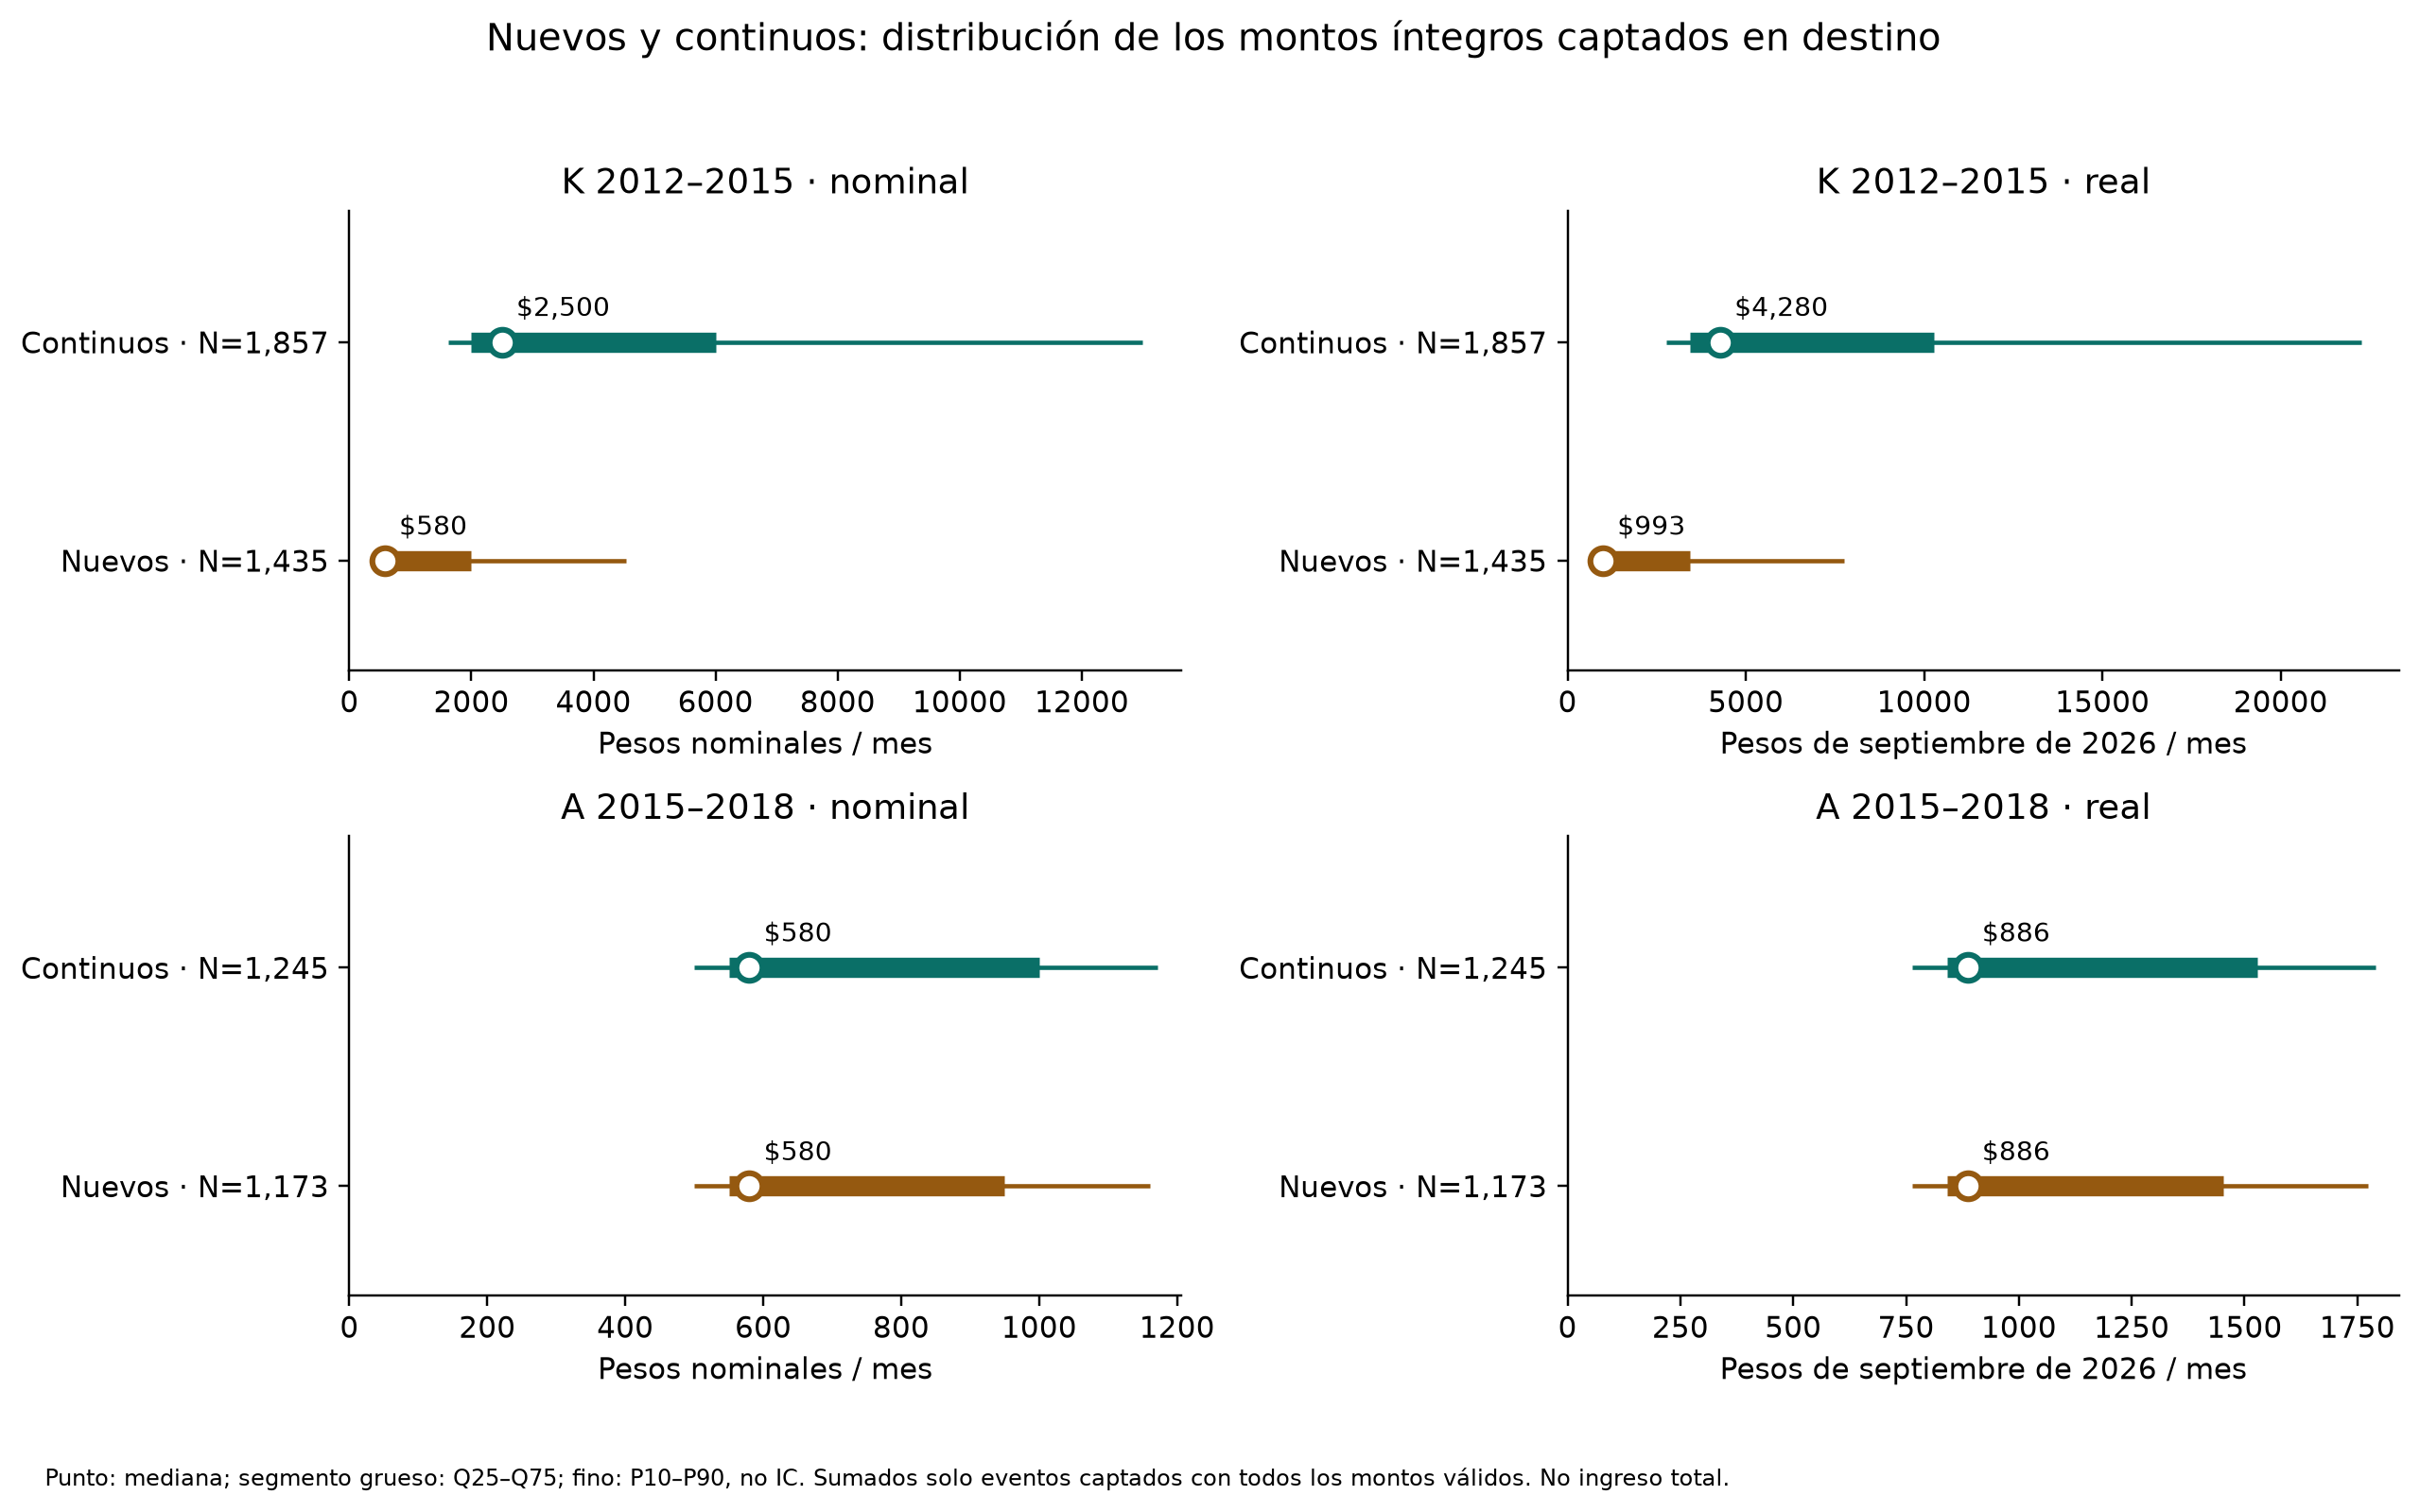
\includegraphics[width=\linewidth,height=.72\textheight,keepaspectratio]{../resultados/figuras/transiciones_montos__nuevos_continuos.png}
\notacuadro{Montos mensuales de destino íntegros entre eventos captados; nuevas respuestas afirmativas y continuidad observadas. N y faltantes en el texto y cuadro~\ref{tab:tesis-incorporacion}. Cuantiles describen dispersión y no sustituyen IC. Comparación K 2012--2015 y A 2015--2018, no una prueba entre programas homogéneos.}
\fuentecuadro{Elaboración propia, agregados longitudinales; Informe General, figura 46. Nominales y pesos de septiembre de 2026.}
\end{figure}
\end{landscape}
\FloatBarrier

Como se documentó en la sección~\ref{sec:resultados-complementariedad},
la incorporación a K o A puede registrarse en quien ya declaraba la otra,
sin acreditar una prestación económica adicional.
La comparación monetaria nuevos--continuos no separa en sí misma los
importes según ese estado basal de complementariedad.

\section{Heterogeneidad institucional}

Con evidencia IMSS/ISSSTE, los nuevos y continuos K tienen ambas medianas
nominales de 2\,500 pesos; el contraste real es
\dato{K.Institucional.IC}, cuyo intervalo incluye cero.
La diferencia entre el contraste total y el del subgrupo solapado es
\dato{K.DiferenciaContrastes.IC}. El remuestreo utiliza las mismas personas
en ambas cantidades, respetando su solapamiento.

La lectura institucional no consiste en que el total K y ese subgrupo
representen regímenes excluyentes. La evidencia puede ser múltiple y el
importe es personal, no separable por institución. El código agrupado8
aparece en 927/1\,435 nuevos con monto y 144/1\,857 continuos.
Esa diferencia acompaña una mezcla institucional distinta, pero no identifica
por sí sola PAM, contributividad o la fracción de una caída atribuible
a política pública.

El contraste grande del conjunto y la coincidencia mediana del subgrupo
limitan una explicación uniforme sobre los receptores K. No prueban que
la institución cause un nivel monetario ni que todos sus miembros tengan
distribuciones iguales. La hipótesis sobre composición gana una descripción
más específica, no una descomposición causal del cambio transversal.

\section{Cambios individuales frente a diferencias transversales}
\label{sec:resultados-cambios}

El cuadro~\ref{tab:tesis-cambios} utiliza \dato{K.Pares} pares K y
\dato{A.Pares} A con importes íntegros captados en ambas visitas.
Son las mismas personas dentro de cada fila. El cambio expresa diferencia
en el monto mensual entre visitas, no una pérdida mensual recurrente ni
una tasa anual.

% Exportado desde agregados; no editar cifras manualmente.
\begin{table}[!htbp]
\centering
\caption{Mediana del cambio real individual entre receptores continuos}\label{tab:tesis-cambios}
\footnotesize\setlength{\tabcolsep}{3pt}\renewcommand{\arraystretch}{1.25}
\begin{tabularx}{\linewidth}{YYYYY}
\toprule
\textbf{Vía y periodo} & \textbf{Criterio} & \textbf{N pares} & \textbf{$\Delta$ [IC95\%]} & \textbf{Por folio [IC95\%]} \\
\midrule
K 2012--2015 & Periodo principal & 1\,756 & \ensuremath{-40,26}\ \allowbreak\ensuremath{[-82,77;\,-19,00]} & \ensuremath{-40,26}\ \allowbreak\ensuremath{[-82,77;\,-19,00]} \\
K 2012--2015 & Doce meses previos & 1\,756 & \ensuremath{-13,59}\ \allowbreak\ensuremath{[-40,84;\,24,75]} & \ensuremath{-13,59}\ \allowbreak\ensuremath{[-40,84;\,24,75]} \\
K 2012--2015 & Año de entrevista & 1\,756 & \ensuremath{5,86}\ \allowbreak\ensuremath{[-30,52;\,34,03]} & \ensuremath{5,86}\ \allowbreak\ensuremath{[-30,52;\,34,03]} \\
A 2015--2018 & Periodo principal & 1\,223 & \ensuremath{-55,02}\ \allowbreak\ensuremath{[-55,02;\,-33,63]} & \ensuremath{-55,02}\ \allowbreak\ensuremath{[-55,02;\,-30,57]} \\
A 2015--2018 & Doce meses previos & 1\,223 & \ensuremath{-68,17}\ \allowbreak\ensuremath{[-72,39;\,-57,79]} & \ensuremath{-68,17}\ \allowbreak\ensuremath{[-73,32;\,-55,11]} \\
A 2015--2018 & Año de entrevista & 1\,223 & \ensuremath{-71,49}\ \allowbreak\ensuremath{[-71,49;\,-57,83]} & \ensuremath{-71,49}\ \allowbreak\ensuremath{[-71,49;\,-57,83]} \\
K 2012--2015 & Un evento; misma contingencia/institución & 1\,183 & \ensuremath{-77,18}\ \allowbreak\ensuremath{[-104,03;\,-39,70]} & \ensuremath{-77,18}\ \allowbreak\ensuremath{[-104,03;\,-35,07]} \\
\bottomrule
\end{tabularx}
\notacuadro{Montos mensuales íntegros captados en ambas visitas; cambio final menos inicial de cada persona. Pesos de septiembre de 2026. Principal: promedio INPC del año anterior a entrevista real; alternativas conservan los mismos pares. Folio cunicah es sensibilidad, no hogar actual o UPM validada. La última fila cambia el universo y no acredita misma prestación administrativa. No se imputan pagos tras fallecimiento.}
\fuentecuadro{Elaboración propia, ENASEM; agregados de notebooks 06--08 y validación focalizada del informe general, secciones 10.2--10.7. Sin ponderación nacional.}
\end{table}

\FloatBarrier

La mediana del cambio K principal es \dato{K.Cambio.IC} pesos reales.
El intervalo es negativo bajo ese criterio, pero la magnitud es pequeña
frente a una dispersión individual Q25/Q75 de
\dato{K.Cambio.q25}/\dato{K.Cambio.q75}.
Con doce meses previos resulta \dato{K.DoceMeses.IC}; con promedio del
año de entrevista, \dato{K.Anual.IC}. Ambos intervalos incluyen cero
y el último puntual cambia de signo. No se sostiene una caída mediana K
robusta a todos los criterios temporales.

En A, la mediana principal es \dato{A.Cambio.IC}, y las alternativas
\dato{A.DoceMeses.IC} y \dato{A.Anual.IC} permanecen negativas.
El signo es más estable dentro de los escenarios examinados.
Sin embargo, Q25/Q75 de cambios
\dato{A.Cambio.q25}/\dato{A.Cambio.q75} muestran heterogeneidad y
aumentos individuales. Las proporciones de cambios negativos son
\dato{K.Negativos.IC}\% y \dato{A.Negativos.IC}\% para K y A;
no representan toda la cohorte inicial.

\begin{landscape}
\begin{figure}[p]
\centering
\caption{Cambios reales individuales y sensibilidades de concepto entre continuos}
\label{fig:tesis-cambios}
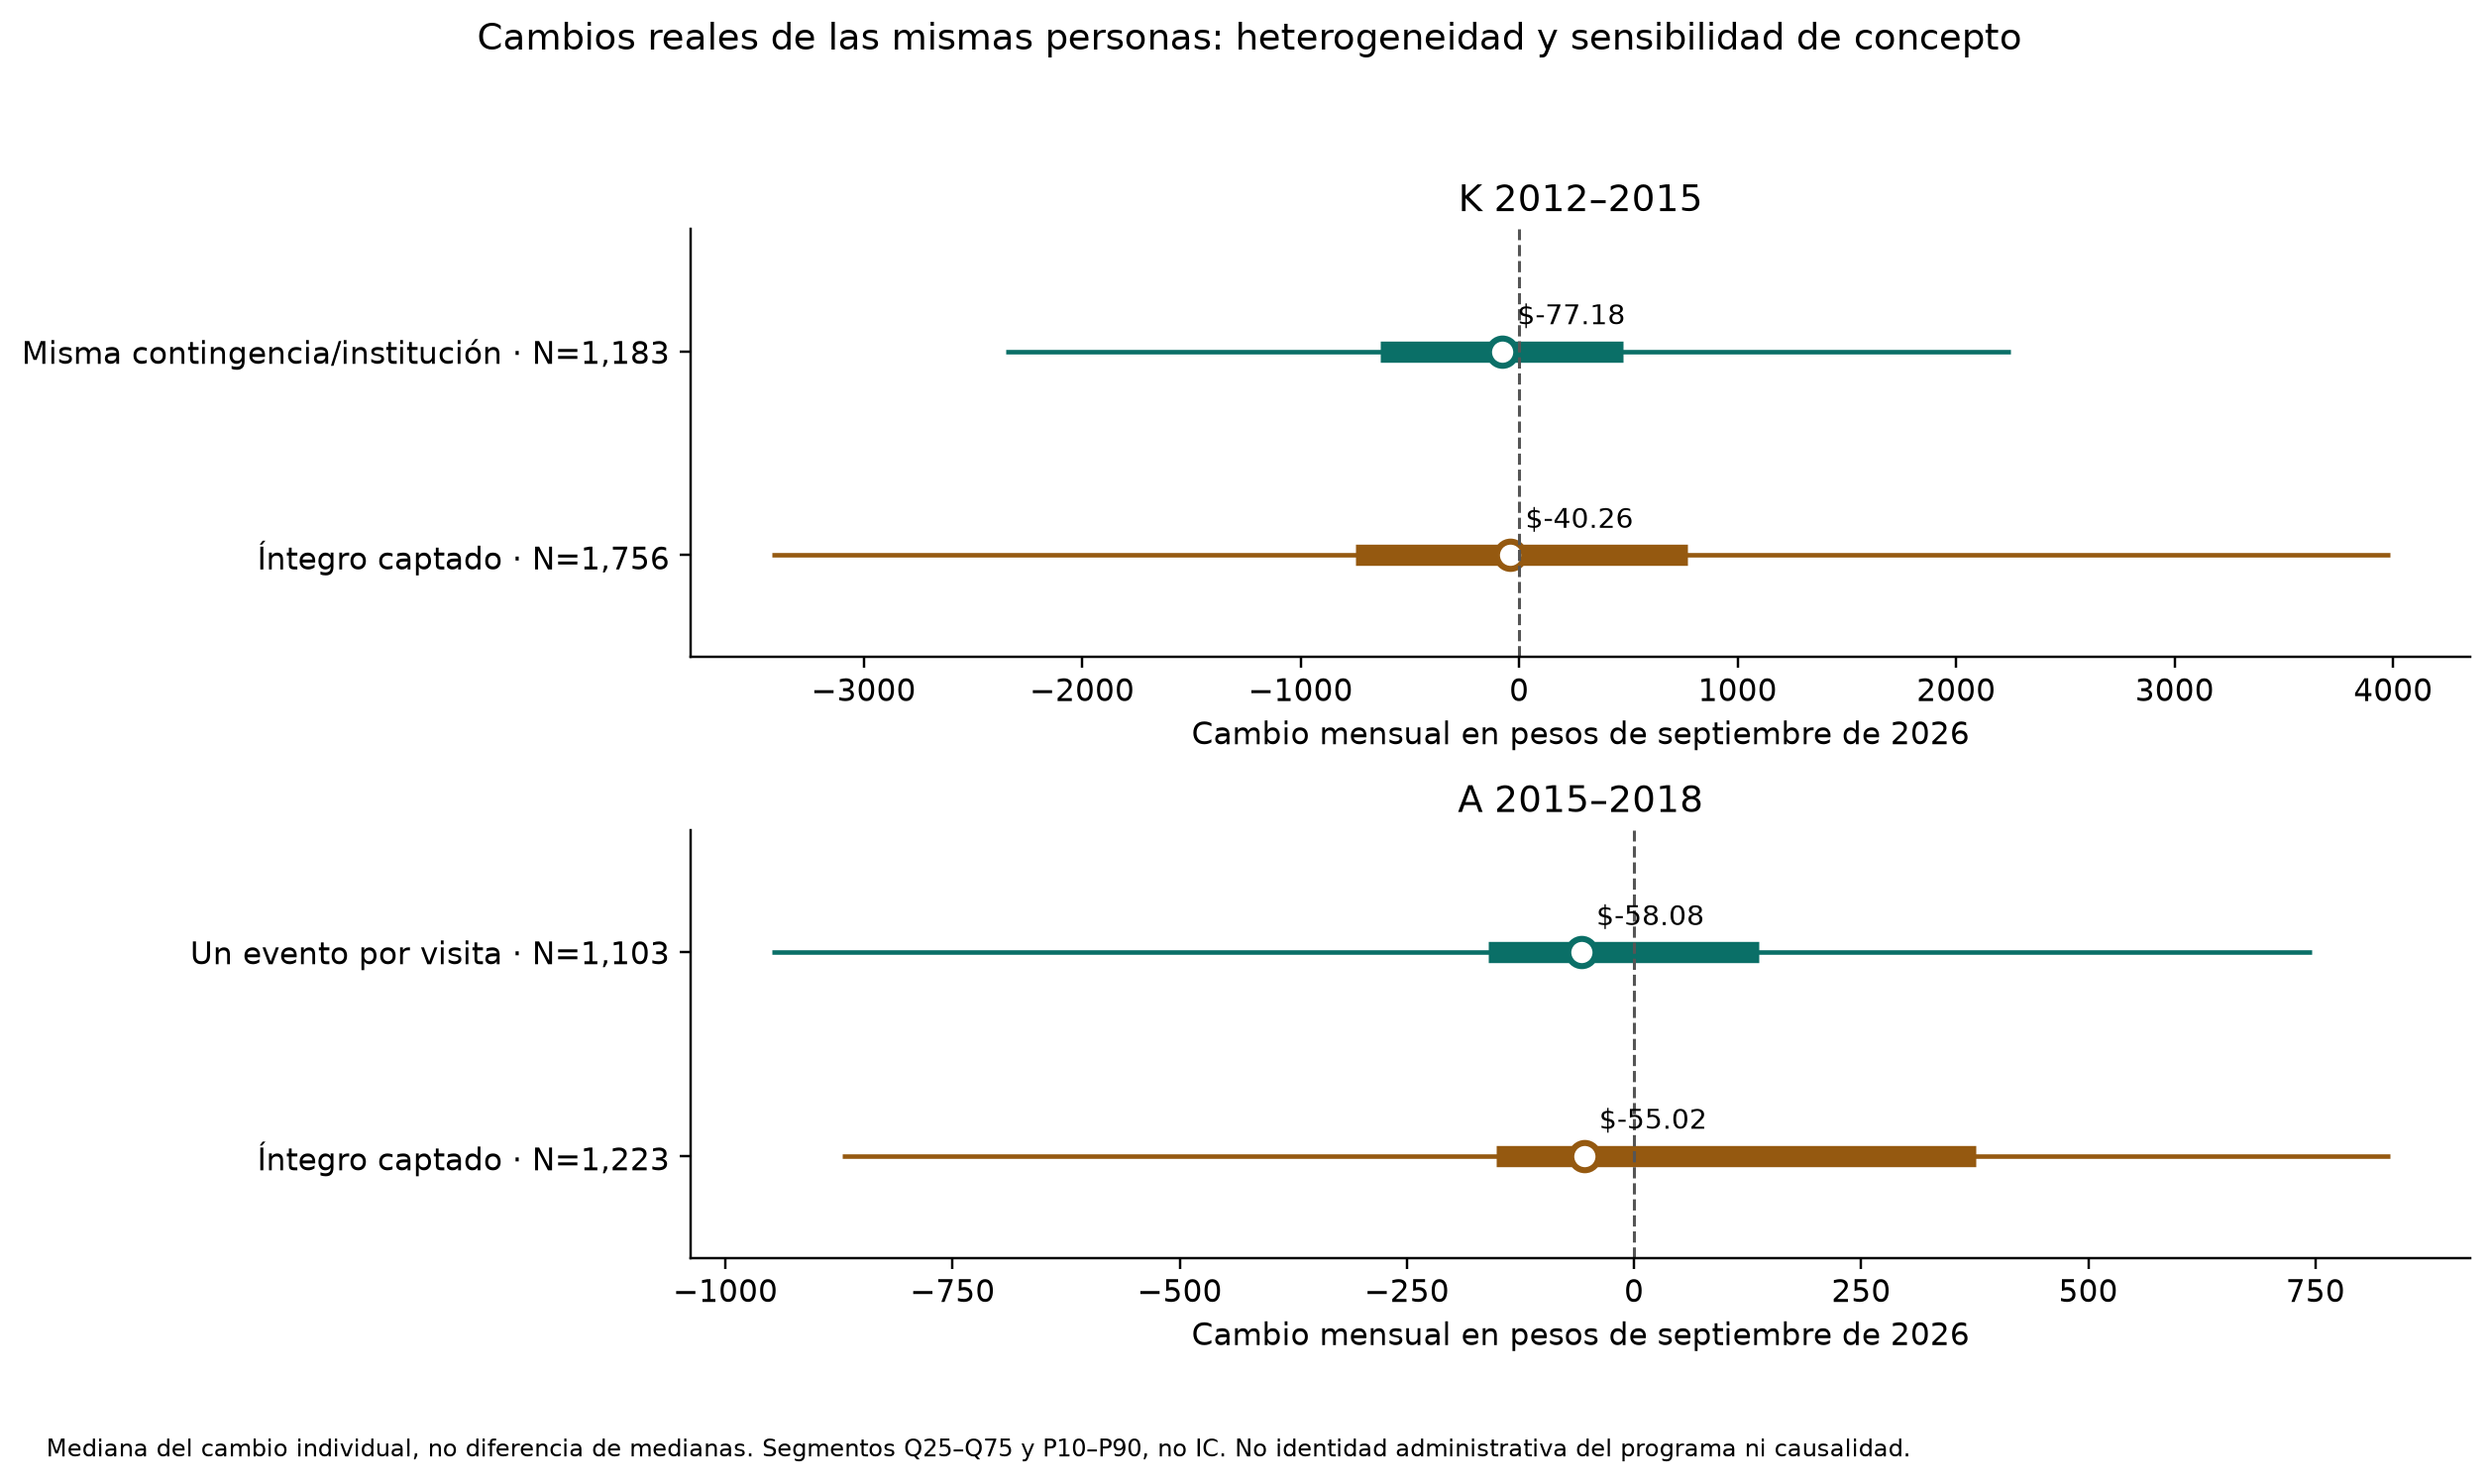
\includegraphics[width=\linewidth,height=.72\textheight,keepaspectratio]{../resultados/figuras/transiciones_montos__cambios_personales.png}
\notacuadro{K 2012--2015 y A 2015--2018; directas 60+ basales. Principal: N=1\,756/1\,223 pares íntegros. Sensibilidades: K con un evento y misma contingencia/institución, N=1\,183; A con un evento por visita, N=1\,103. Estas restricciones cambian la población y no acreditan identidad administrativa. Las barras son cuantiles del cambio, no IC; la precisión de los contrastes seleccionados aparece en el cuadro~\ref{tab:tesis-cambios}.}
\fuentecuadro{Elaboración propia, agregados longitudinales e Informe General, figura 47. Pesos mensuales de septiembre de 2026.}
\end{figure}
\end{landscape}
\FloatBarrier

Quedan \dato{K.SinCambio} continuos K y \dato{A.SinCambio} A sin cambio
calculable entre todos los Sí$\rightarrow$Sí conocidos. Las cotas externas
de mediana que admiten posiciones extremas de sus cambios faltantes son
\dato{K.CotaCambio} y \dato{A.CotaCambio}, respectivamente.
K puede cruzar cero; A conserva signo negativo bajo el criterio temporal
principal de ese ejercicio. Son cotas de información incompleta, no
intervalos conjuntos de muestreo y faltantes. No incluyen a personas
fallecidas o ausentes.

\section{Sensibilidad a mortalidad y pérdida de seguimiento}
\label{sec:resultados-seleccion}

De la cohorte basal K de \dato{K.Basal} personas, se registran
\dato{K.Muertes} fallecimientos, \dato{K.Ausencias} ausencias de estado
vital desconocido y \dato{K.Sustitutos} sustitutos vivos en destino.
Para A, entre \dato{A.Basal}, los conteos son
\dato{A.Muertes}, \dato{A.Ausencias} y \dato{A.Sustitutos}.
Un conflicto vital A se mantiene separado del principal.
No se suman estos destinos a las negativas de recepción.

Los agregados de seguimiento muestran diferencias según recepción basal,
pero la dirección de la ausencia no es uniforme entre vías.
La cohorte inicial y los pares monetarios observados responden, por ello,
a poblaciones diferentes. Las reapariciones posteriores confirman que
ausencia no equivale a muerte ni a pérdida definitiva.

Permitir sustitutos válidos en destino mantiene las medianas generales
de nuevos y continuos K/A con N mayores, sin acreditar ausencia de sesgo
en los subgrupos. Estandarizar composición de observados tampoco recupera
los importes de quienes no se observan. La mortalidad completa, la selección
no observada y los montos de toda la cohorte siguen sin identificarse.
No se ofrecen trayectorias imputadas después del fallecimiento ni una
corrección por probabilidad de observación.

\section{Síntesis de resultados frente a la hipótesis}
\label{sec:resultados-sintesis}

H1 encuentra respaldo localizado: en K 2012--2015 y A 2015--2018,
mayor recepción coincide con menor mediana real transversal.
El aumento real K 2018--2021 impide extender esa lectura a todo el periodo.
Además, la comparación transversal no describe la pérdida personal de
todos los receptores.

Para H2, el contraste K entre nuevos y continuos es grande en la definición
original y persiste bajo composición común, pero su magnitud se reduce
sustancialmente bajo la sensibilidad institucional; su lectura cambia al examinar evidencia
IMSS/ISSSTE. A presenta el nulo mediano relevante. Las ventanas y conceptos
son diferentes: no se ha estimado un efecto común ni una interacción
causal entre programas.

H3 es consistente con la reducción de brecha de unión y con brechas de
monto positivas en los dos cortes. No se establece con precisión el
ensanchamiento monetario. La figura~\ref{fig:tesis-precision} reúne la
precisión de los contrastes y muestra dónde los intervalos incluyen cero.

\begin{landscape}
\begin{figure}[p]
\centering
\caption{Precisión condicional de incorporación, continuidad y brechas por sexo}
\label{fig:tesis-precision}
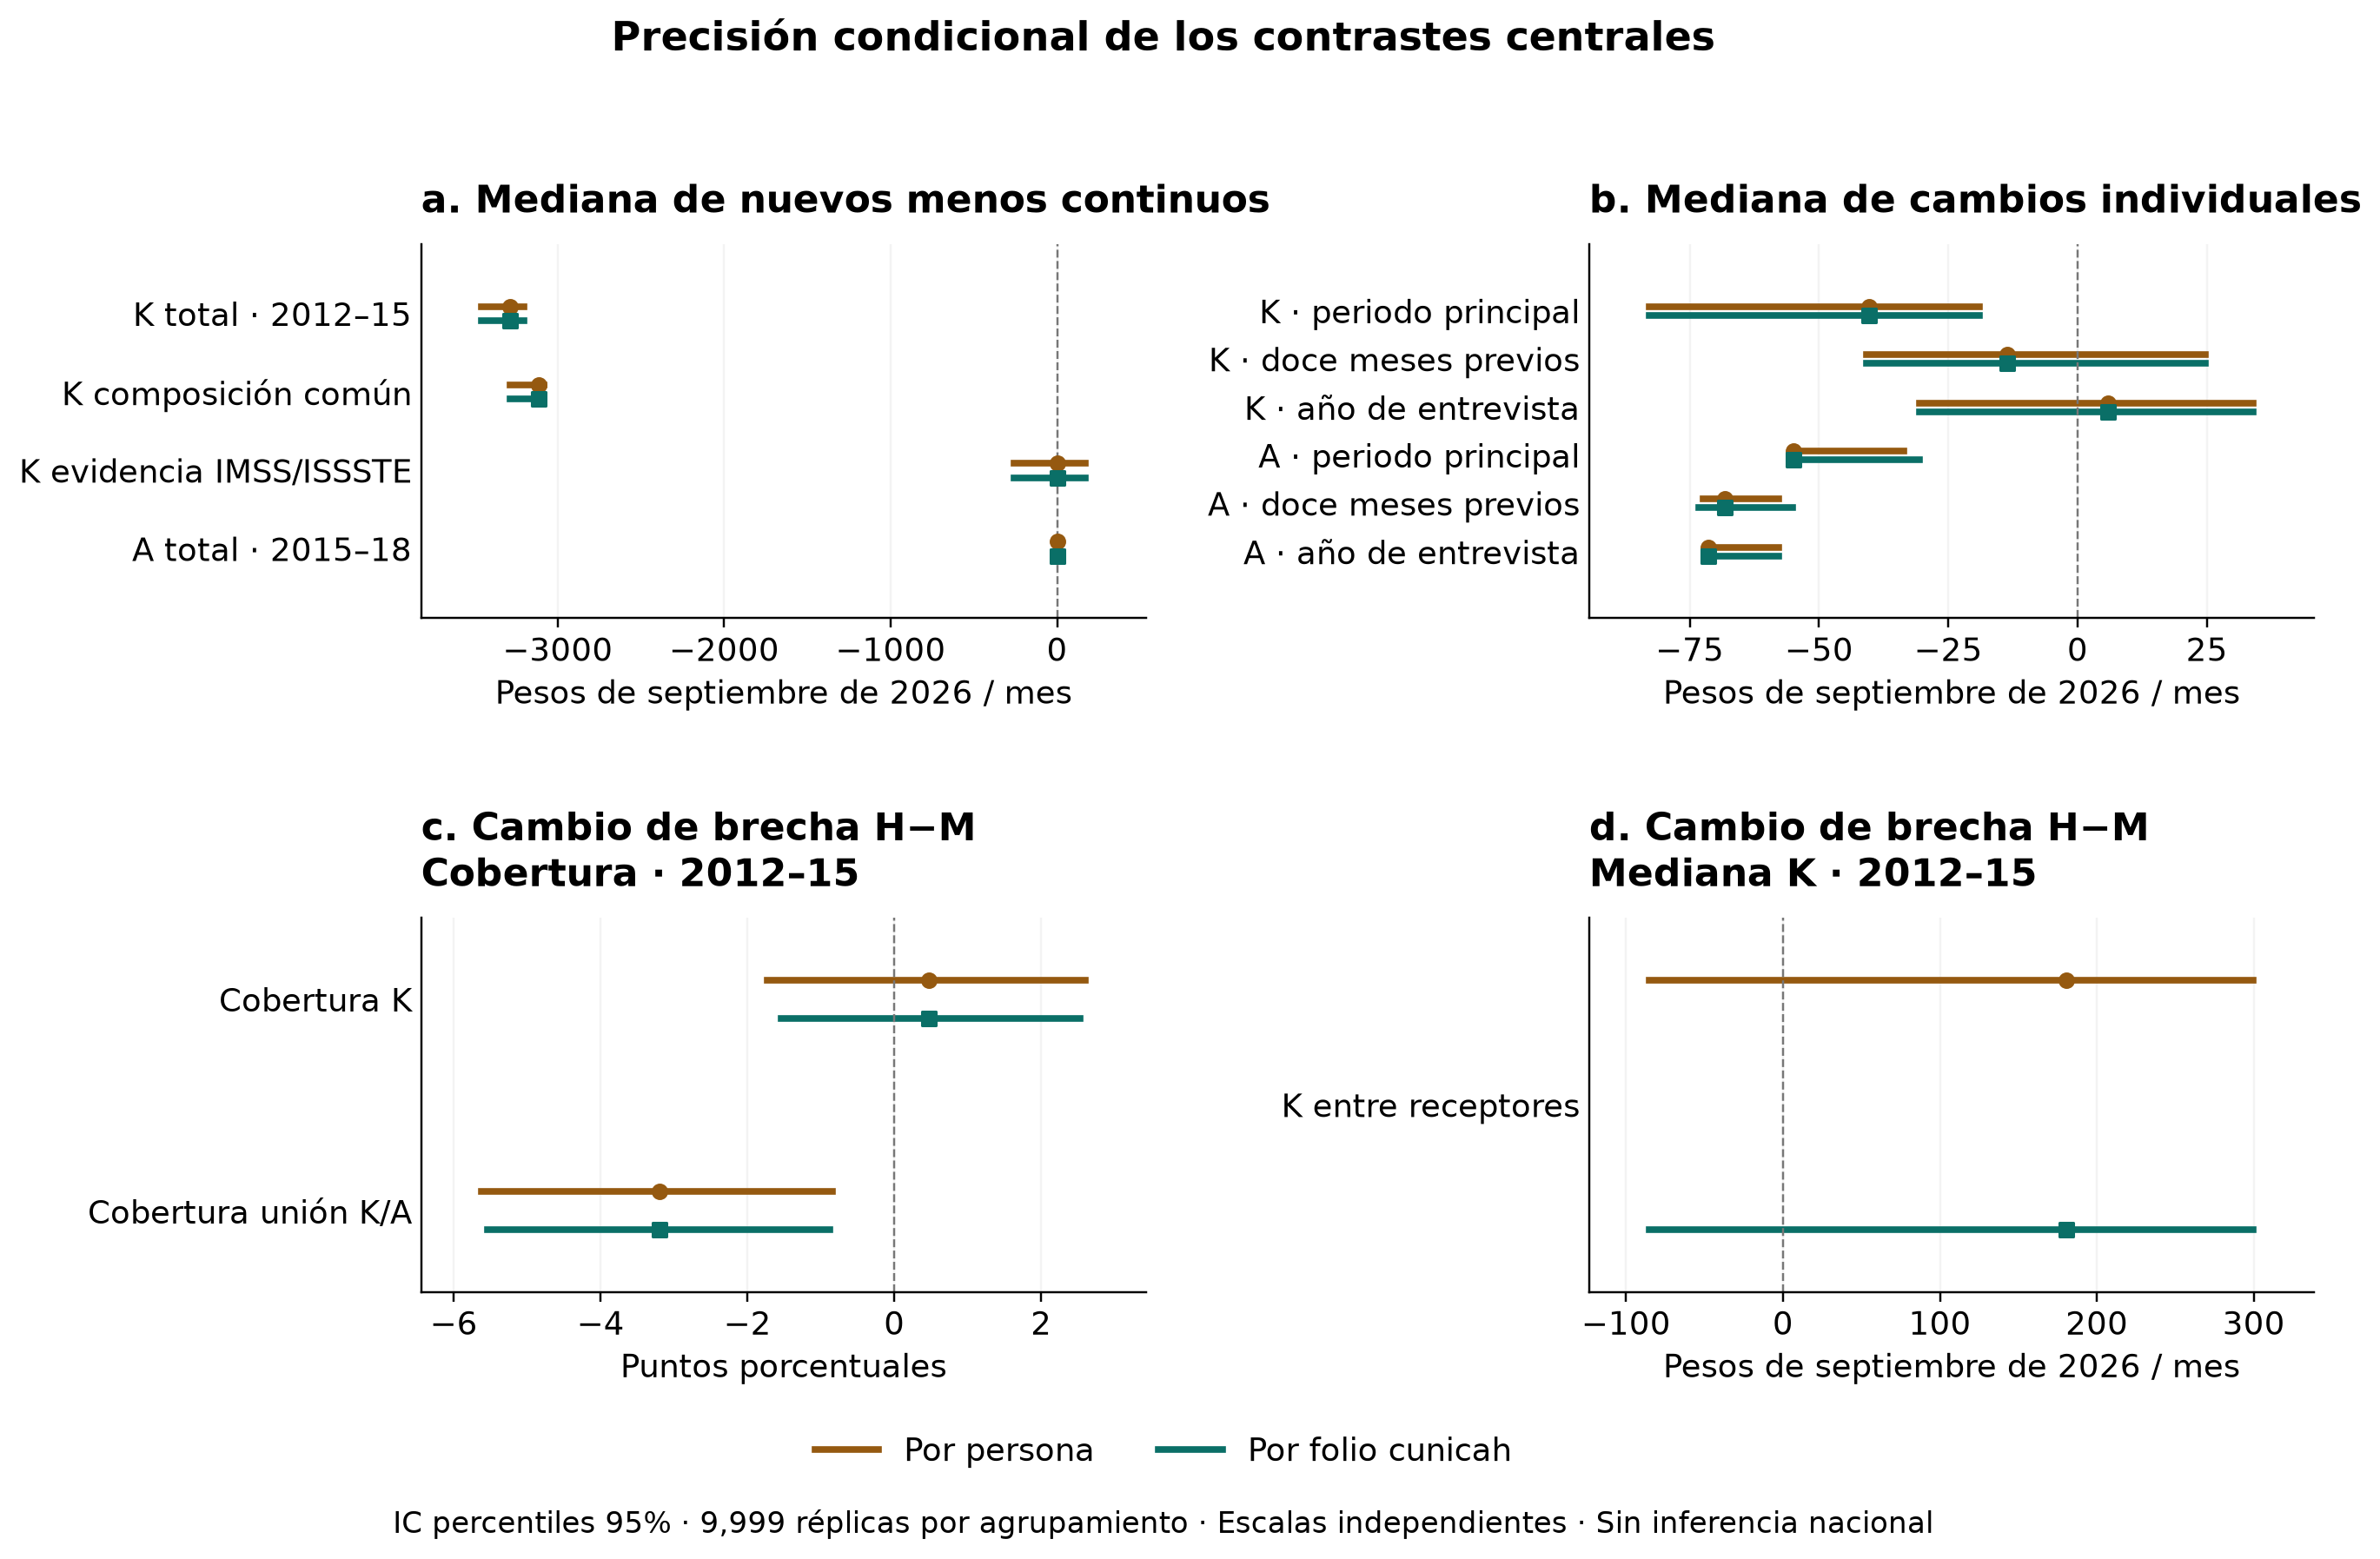
\includegraphics[width=\linewidth,height=.72\textheight,keepaspectratio]{../resultados/figuras/transiciones_montos__precision.png}
\notacuadro{IC percentiles 95\%, 9\,999 réplicas por persona y sensibilidad por folio. Paneles de incorporación: montos de destino; cambios individuales: pares K/A; brechas: cortes dinámicos2012/2015. Las escalas de pesos y puntos porcentuales difieren por panel. N en cuadros~\ref{tab:tesis-incorporacion}--\ref{tab:tesis-cambios} y~\ref{tab:tesis-sexo}. No hay inferencia de diseño nacional.}
\fuentecuadro{Validación focalizada reproducible de los agregados06--08; Informe General, figura 48 y sección 10.7. Pesos de septiembre de 2026.}
\end{figure}
\end{landscape}
\FloatBarrier

El balance respalda una relación no uniforme entre ampliación de acceso
y niveles de recursos captados, acotada a las definiciones y ventanas
verificadas; no identifica una mejora del ingreso total.
La precisión muestral refuerza algunos contrastes y limita otros;
no convierte la hipótesis general en una conclusión nacional demostrada
ni identifica mecanismos causales de política pública.



% BEGIN calidad10
\section{Calidad del soporte y robustez de las comparaciones}
\label{sec:resultados-calidad10}

K 2001--2003 no permite una conclusión monetaria direccional P/C: C tiene
11 montos válidos y dividirlo en cuartiles genera ramas de muy baja frecuencia.
Las mitades patrimoniales no rescatan ese soporte. Se conservan sus originales
privados y el no estimado; no se agrupan ventanas para obtener precisión.

\begingroup\small\setlength{\tabcolsep}{3pt}
\begin{longtable}{lrrrp{.21\textwidth}}
\caption{Precisión monetaria P menos C y estabilidad de remuestreo}\label{tab:calidad-tesis_calidad_precision}\\
\toprule
Vía/ventana & N P/C & IC semilla1 & IC semilla2 & Evaluación \\
\midrule\endfirsthead
\multicolumn{5}{l}{Continuación del cuadro \thetable}\\
\toprule
Vía/ventana & N P/C & IC semilla1 & IC semilla2 & Evaluación \\
\midrule\endhead
\bottomrule\endfoot
K 2001--2003 & 278/11 & No confiable & No confiable & Sin soporte direccional \\
K 2012--2015 & 1,060/373 & [51.4; 668.3] & [51.4; 409.1] & Dirección cruda estable \\
K 2018--2021 & 360/132 & [543.9; 1,324.3] & [543.9; 1,281.3] & Dirección cruda estable \\
A 2003--2012 & 666/98 & [0.0; 0.0] & [0.0; 0.0] & Condicional; empates \\
A 2012--2015 & 1,196/286 & [0.0; 0.0] & [0.0; 0.0] & Condicional; empates \\
A 2015--2018 & 581/589 & [-30.6; 7.6] & [-30.6; 7.6] & Medianas coincidentes \\
\end{longtable}
{\footnotesize Fuente: auditoría10, insumos01--09 intactos. Muestra sin ponderación; IC condicionales, sin inferencia nacional o causal. P: primera vía observada; C: otra vía basal afirmativa. 9999 réplicas por folio y dos semillas. Se muestran estimación e IC. Los intervalos por orden e influencia están en el informe. La diferencia K2001--2003 no se usa como conclusión direccional aunque pueda calcularse.\par}
\endgroup

\begingroup\small\setlength{\tabcolsep}{3pt}
\begin{longtable}{lrrr}
\caption{Sensibilidad del gradiente patrimonial de incorporación}\label{tab:calidad-tesis_calidad_gradiente}\\
\toprule
Vía/ventana & Edad3/celda20 pp & Edad2/celda30 pp & N soporte Q1/Q4 \\
\midrule\endfirsthead
\multicolumn{4}{l}{Continuación del cuadro \thetable}\\
\toprule
Vía/ventana & Edad3/celda20 pp & Edad2/celda30 pp & N soporte Q1/Q4 \\
\midrule\endhead
\bottomrule\endfoot
K 2001--2003 & -0.5 [-3.1; 1.9] & -0.8 [-3.2; 1.7] & 956/831 \\
K 2012--2015 & 0.5 [-4.0; 5.0] & 0.3 [-4.2; 4.9] & 918/894 \\
K 2018--2021 & -4.0 [-7.7; -0.4] & -4.0 [-7.6; -0.4] & 668/596 \\
A 2003--2012 & 6.8 [0.3; 13.2] & 6.9 [0.9; 13.3] & 527/499 \\
A 2012--2015 & 4.0 [-0.8; 8.6] & 4.0 [-1.0; 8.8] & 919/895 \\
A 2015--2018 & 6.2 [0.7; 11.6] & 4.7 [-0.8; 10.2] & 508/490 \\
\end{longtable}
{\footnotesize Fuente: auditoría10, insumos01--09 intactos. Muestra sin ponderación; IC condicionales, sin inferencia nacional o causal. P: primera vía observada; C: otra vía basal afirmativa. Q1 menos Q4 entre negativas K/A reobservadas; sexo y escolaridad se mantienen. Edad2=60--69/70+, edad3=60--64/65--69/70+. Cambian soporte y mezcla, no es la misma población. Todas las cuatro especificaciones están en el informe; no se elige por significancia.\par}
\endgroup


Los cuadros registran todas las variantes, sin escoger las que excluyen cero.
A 2003--2012 mantiene gradiente positivo en las especificaciones viables,
pero A 2015--2018 y K 2018--2021 dependen del soporte; A 2012--2015 incluye
cero tras ajuste. Los P--C K recientes conservan dirección cruda con dos
semillas, pero el extremo superior K 2012--2015 es inestable. La robustez
al remuestreo no implica robustez a la medición institucional. Los empates A
se conservan sin inferir equivalencia.

\begingroup\small\setlength{\tabcolsep}{3pt}
\begin{longtable}{lp{.26\textwidth}rrp{.15\textwidth}}
\caption{Soporte de los contrastes institucionales P menos C}\label{tab:calidad-tesis_calidad_instituciones}\\
\toprule
Vía/ventana & Institución & N P/C & Diferencia [IC95] & Uso \\
\midrule\endfirsthead
\multicolumn{5}{l}{Continuación del cuadro \thetable}\\
\toprule
Vía/ventana & Institución & N P/C & Diferencia [IC95] & Uso \\
\midrule\endhead
\bottomrule\endfoot
K 2001--2003 & Evidencia IMSS/ISSSTE & 244/$<$10 & No estimable & No confiable \\
K 2001--2003 & Programas agrupados & 0/0 & No estimable & No confiable \\
K 2001--2003 & Un evento IMSS & 214/$<$10 & No estimable & No confiable \\
K 2001--2003 & Un evento ISSSTE & 25/$<$10 & No estimable & No confiable \\
K 2012--2015 & Evidencia IMSS/ISSSTE & 406/27 & 513.5 [0.0; 1,027.1] & Exploratorio 10--29 \\
K 2012--2015 & Programas agrupados & 599/326 & 0.0 [0.0; 0.0] & Sin equivalencia \\
K 2012--2015 & Un evento IMSS & 305/20 & 428.0 [0.0; 684.7] & Exploratorio 10--29 \\
K 2012--2015 & Un evento ISSSTE & 63/$<$10 & No estimable & No confiable \\
K 2018--2021 & Evidencia IMSS/ISSSTE & 309/79 & 679.9 [-61.2; 1,087.8] & Exploratorio \\
K 2018--2021 & Programas agrupados & 0/0 & No estimable & No confiable \\
K 2018--2021 & Un evento IMSS & 259/68 & 271.9 [-192.4; 679.9] & Exploratorio \\
K 2018--2021 & Un evento ISSSTE & 33/10 & No estimable & No confiable \\
\end{longtable}
{\footnotesize Fuente: auditoría10, insumos01--09 intactos. Muestra sin ponderación; IC condicionales, sin inferencia nacional o causal. P: primera vía observada; C: otra vía basal afirmativa. Conteos monetarios pequeños se indican como menos de10. Las ramas con10--29 se revisaron por amplitud e influencia: las viables se conservan como exploratorias, incluyan o no cero. Las no confiables se indican sin estimación. No se mezclan instituciones para obtener N. Sin programa común longitudinalA.\par}
\endgroup


Institución y evento único reducen el soporte; las ramas de 20--29 válidos
C son exploratorias y las insuficientes no se usan para concluir dirección.
La comparación siguiente es contexto transversal por escolaridad agrupada,
no una respuesta causal ni longitudinal. Su universo de 60+ incluye modalidades
distintas de la muestra directa principal; ND se conserva como información
insuficiente, no como perfil económico.
\begingroup\small\setlength{\tabcolsep}{3pt}
\begin{longtable}{lrrrrr}
\caption{Reformulación del contexto patrimonial por escolaridad y titularidad,2021}\label{tab:calidad-tesis_calidad_T8}\\
\toprule
Titularidad K & Esc. años & N & Q25 & Mediana & Q75 \\
\midrule\endfirsthead
\multicolumn{6}{l}{Continuación del cuadro \thetable}\\
\toprule
Titularidad K & Esc. años & N & Q25 & Mediana & Q75 \\
\midrule\endhead
\bottomrule\endfoot
Ambas & 0--5 & 84 & 419.9 & 805.6 & 1,088.3 \\
Ambas & 6+ & 384 & 800.0 & 1,580.0 & 2,769.7 \\
Ambas negativas K & 0--5 & 3,251 & 90.0 & 450.0 & 1,000.0 \\
Ambas negativas K & 6+ & 2,377 & 152.0 & 650.0 & 1,382.7 \\
Solo cónyuge & 0--5 & 385 & 400.0 & 800.0 & 1,505.0 \\
Solo cónyuge & 6+ & 677 & 530.0 & 1,050.0 & 2,022.0 \\
Solo propia & 0--5 & 996 & 224.9 & 650.8 & 1,222.5 \\
Solo propia & 6+ & 2,067 & 400.0 & 914.3 & 1,800.7 \\
\end{longtable}
{\footnotesize Fuente: EDA original60+ por visita, incluidas modalidades originales; no es la población principal directa09. Patrimonio compartido, miles de unidades almacenadas, no pesos reales. Escolaridad0--5/6+; titularidad o escolaridad ND quedan como exclusiones. Se presentan todos los grupos, no máximos seleccionados.\par}
\endgroup

% END calidad10
